\chapter{Hypergraph Symmetry and \FKA{} Recursion}

\section{Symmetries in Hypergraphs}\label{sec:symmetries}

\begin{definition}
A \emph{permutation} of the vertex set $V$ of a hypergraph $H=(V,E)$ is a bijection of $V$. A \emph{permutation group} $\mathcal{G}$ on $H$ is a set of permutations $\alpha,\omega,\chi,\gamma,\dots$ of $V$ such that:
\begin{enumerate}
\item $\mathcal{G}$ contains the trivial permutation.
\item $\mathcal{G}$ contains $\alpha^{-1}$ for every $\alpha\in\mathcal{G}$, where $\alpha^{-1}(\alpha(v))=v$ for all $v\in V$.
\item $\mathcal{G}$ is closed under composition: $(\alpha\circ\omega)(v)=\alpha(\omega(v))$ for all $\alpha,\omega\in\mathcal{G}$ and $v\in V$.
\end{enumerate}
Each $\alpha\in\mathcal{G}$ maps edges $e\in E(H)$ to edges $\alpha(e)=\{\alpha(v)\mid v\in e\}$, and non-edges to non-edges, preserving the structure of $H$.
\end{definition}

\begin{definition}
Two hypergraphs $H=(V,E)$ and $H'=(V',E')$ are \emph{isomorphic} if there exists a bijection $\lambda:V\to V'$ such that for every edge $e\in E$, the image $\lambda(e)=\{\lambda(v)\mid v\in e\}$ is an edge in $E'$. Formally,
\[
H\cong H'\iff\exists\lambda:V\to V'\text{ bijective},\ \forall e\in E,\ \lambda(e)\in E'.
\]
\end{definition}

\begin{definition}
An \emph{automorphism} of a hypergraph $H=(V,E)$ is an isomorphism from $H$ to itself. The \emph{automorphism group} $\Aut(H)$ of $H$ is the set of all automorphisms of $H$ under composition.
\end{definition}

Consider the hypergraphs $G$ where $G=\{\{v_1,v_5,v_6\},\{v_4,v_5,v_6\},\{v_1,v_2\},\{v_2,v_3,v_4\}\}$. The automorphism group of the hypergraph is : $\Aut(H)=\langle(v_1\ v_4),(v_5\ v_6)\rangle$, which is isomorphic to $C_2\times C_2$.

Most hypergraphs are asymmetric, meaning they lack nontrivial automorphisms. However, hypergraphs can exhibit localized symmetry in their induced subhypergraphs, even when the global structure remains asymmetric. It is well known that while every abstract group can be realized as the full automorphism group of a graph, not every permutation group can. Hence, the question of whether a given permutation group $\mathcal{G}$ acting on $\{v_1,\dots,v_n\}$ can serve as the automorphism group of a hypergraph with vertex set $\{v_1,\dots,v_n\}$ has been extensively studied and classified for some class of groups. Whether the existence of such symmetries plays any role in the \FKA{} performance remains unknown.

\begin{definition}
Given a graph or hypergraph $H=(V,E)$ and an automorphism group $\mathcal{G}$ acting on the vertex set $V$, the \emph{orbit} of a vertex $v\in V$ under $\mathcal{G}$ is the set:
\[
O(v)=\{g(v)\mid g\in\mathcal{G}\}
\]
consisting of all vertices that $v$ can be mapped to by the automorphisms in $\mathcal{G}$.
\end{definition}

\begin{definition}
A \emph{partition} of the vertex set $V$ of a hypergraph $H=(V,E)$ is a collection of disjoint subsets $V_1,V_2,\dots,V_k$ such that:
\[
V=\bigcup_{i=1}^{k}V_i\quad\text{and}\quad V_i\cap V_j=\emptyset\text{ for all }i\neq j.
\]
Each subset $V_i$ is called a \emph{partition class}.
\end{definition}

Each orbit partitions the vertex set $V$ into equivalence classes permuted by automorphisms $g\in\Aut(H)$. Nontrivial vertex permutations are referred to as automorphism \emph{generators} when they are elements of the automorphism group that generate all other group elements under composition. The set of generators, through their action on the vertex set $V$, precisely determine and generate the orbits.

\begin{claim}
The vertex sets of the subhypergraphs of $H$ under the automorphism group $\mathcal{G}=\Aut(H)$ are precisely the orbits of the action of $\mathcal{G}$ on $V$. \cite{Lec}
\end{claim}

\begin{proof}
Let $O(v_i)=\{\sigma(v_i)\mid\sigma\in\mathcal{G}\}$ be the orbit of a vertex $v_i\in V$ under the action of $\mathcal{G}$. By definition, the orbit $O(v_i)$ is closed under the action of $\mathcal{G}$ since, for any $\sigma,\tau\in\mathcal{G}$ and $v_j\in O(v_i)$ with $v_j=\sigma(v_i)$, we have $\tau(v_j)=\tau(\sigma(v_i))=(\tau\circ\sigma)(v_i)\in O(v_i)$. Thus, $O(v_i)$ forms a stable subset under $\mathcal{G}$, and the vertices of $O(v_i)$ define a subhypergraph of $H$.

Conversely, let $S\subseteq V$ be the vertex set of a subhypergraph of $H$ under $\mathcal{G}$. Since $S$ is closed under the automorphisms in $\mathcal{G}$, for every $\sigma\in\mathcal{G}$ and $s\in S$, we have $\sigma(s)\in S$. For any vertex $s\in S$, its orbit $O(s)=\{\sigma(s)\mid\sigma\in\mathcal{G}\}$ is entirely contained within $S$, as $S$ is closed under the action. Furthermore, $S$ must be a union of orbits because it cannot partially include any orbit without violating closure under $\mathcal{G}$.

Therefore, each orbit under $\mathcal{G}$ corresponds to a subhypergraph of $H$, and any subhypergraph is a union of orbits. Thus, the vertex sets of the subhypergraphs of $H$ are precisely the orbits of the action of $\mathcal{G}$ on $V$.
\end{proof}

A permutation group $\mathcal{G}$ acts \emph{transitively} on the vertices of a hypergraph $H=(V,E)$ if for any two vertices $u,v\in V$, there exists $g\in\mathcal{G}$ such that $g(u)=v$, ensuring uniform symmetry across $V$. A permutation group $\mathcal{G}$ of degree $n$ is said to be \emph{set-transitive} if any two subsets of the vertex set of same cardinality lie in the same orbit of $\mathcal{G}$. If $\mathcal{G}$ is set-transitive, then any $\mathcal{G}$-invariant hypergraph consists of either all or none of the $k$-subsets for all $k$, and its full automorphism group is the symmetric group $S_n$.

In contrast, an action of a permutation group $\mathcal{G}$ on a set $V$ is \emph{intransitive} if $\mathcal{G}$ does not act transitively on $V$, meaning there exist subsets of $V$ that are not connected by the action of $\mathcal{G}$. In this case, $V$ can be partitioned into orbits such that $\mathcal{G}$ acts transitively within each orbit but not across orbits.

\begin{definition}
Let $\mathcal{G}$ be a permutation group acting transitively on the vertex set $V$ of a hypergraph $H=(V,E)$. A subset of vertices $B\subseteq V$ is called a \emph{block} of $\mathcal{G}$ if, for every $g\in\mathcal{G}$, either $g(B)=B$ or $g(B)\cap B=\emptyset$. The blocks of $\mathcal{G}$ form a $\mathcal{G}$-invariant partition of $V$.
\end{definition}

\begin{definition}
A transitive permutation group $\mathcal{G}$ acting on the vertices $V$ of a hypergraph $H$ is called \emph{primitive} if its only blocks are $V$ itself or singletons (i.e., individual vertices).
\end{definition}

\begin{definition}
A transitive permutation group $\mathcal{G}$ acting on the vertices $V$ of a hypergraph $H$ is called \emph{imprimitive} if it admits at least one block that is neither $V$ nor a singleton, resulting in a non-trivial partition of $V$.
\end{definition}

Now we can describe how these groups act on hypergraphs as their automorphism groups.

Let $\mathcal{G}_1$ and $\mathcal{G}_2$ be the automorphism groups of hypergraphs $H_1=(V_1,E_1)$ and $H_2=(V_2,E_2)$, where $V_1$ and $V_2$ are disjoint vertex sets. The \emph{direct product} $\mathcal{G}_1\times\mathcal{G}_2$ acts on the combined hypergraph $H=(V_1\cup V_2,E_1\cup E_2)$, where $E_1\cap E_2=\emptyset$. The action is intransitive, as $\mathcal{G}_1$ and $\mathcal{G}_2$ independently permute vertices within $V_1$ and $V_2$, preserving the disjoint structure of the vertex sets.

For a hyperedge $e\in E$, we have:
\[
((u_1,v_1),\dots,(u_k,v_k))\in e\text{ if and only if }(u_1,\dots,u_k)\in E_1\text{ and }(v_1,\dots,v_k)\in E_2,
\]
and the group action is defined as:
\[
e^{\mathcal{G}}((u_1,v_1),\dots,(u_k,v_k))=(g_1(u_1,\dots,u_k),g_2(v_1,\dots,v_k)),
\]
where $g_1\in\mathcal{G}_1$ and $g_2\in\mathcal{G}_2$.

Whereas the semidirect product $\mathcal{N}\rtimes_\theta\mathcal{K}$ generalizes this structure by combining two groups $\mathcal{N}$ and $\mathcal{K}$ with an additional homomorphism $\theta$ controlling how $\mathcal{K}$ acts on $\mathcal{N}$. When $\theta$ is trivial, the semidirect product reduces to the direct product. Within $\mathcal{G}=\mathcal{N}\rtimes_\theta\mathcal{K}$, the subgroups $\mathcal{N}^*=\{(u,1)\mid u\in\mathcal{N}\}$ and $\mathcal{K}^*=\{(1,x)\mid x\in\mathcal{K}\}$ are isomorphic to $\mathcal{N}$ and $\mathcal{K}$, respectively, and satisfy the properties:
\begin{itemize}
\item $\mathcal{G}=\mathcal{N}^*\mathcal{K}^*$,
\item $\mathcal{N}^*\cap\mathcal{K}^*=\{(1,1)\}$,
\item $\mathcal{N}^*\lhd\mathcal{G}$.
\end{itemize}

The non-trivial blocks created by an imprimitive group capture localized symmetry within the hypergraph. Within each block, the vertices have an induced symmetry on them, defined by $\mathcal{G}$, but the symmetry does not extend uniformly across all vertices in the hypergraph. These localized symmetries create a hierarchical structure, with symmetries operating both within blocks and between blocks, leading to a modular or layered symmetry pattern in the hypergraph. \cite{BCW24}

\begin{definition}
Let $\mathcal{G}_1$ and $\mathcal{G}_2$ be groups, where $\mathcal{G}_2$ acts on a set of vertices $V_1\subseteq V$. Define $\mathcal{N}:=\mathcal{G}_1^{V_1}$, the direct product of copies of $\mathcal{G}_1$ indexed by elements of $V_1$. For each $j\in\mathcal{G}_2$ and $n\in\mathcal{N}$, the map $(n_v)_{v\in V_1}\mapsto(n_{j^{-1}(v)})_{v\in V_1}$ defines an automorphism of $\mathcal{N}$. The homomorphism $\theta$ from $\mathcal{G}_2$ to $\Aut(\mathcal{N})$ maps $j\in\mathcal{G}_2$ to this automorphism. The \emph{wreath product} $\mathcal{G}_1\wr\mathcal{G}_2$ is defined as the semidirect product $\mathcal{N}\rtimes_\theta\mathcal{G}_2$.
\end{definition}

Let $\mathcal{G}_1$ act on $V_2\subseteq V$ and $\mathcal{G}_2$ on $V_1\subseteq V$. Then $\mathcal{G}_1\wr\mathcal{G}_2$ acts on $V_2\times V_1$ as:
\[
(n,j)\cdot(v_2,v_1):=(n_{j(v_1)}(v_2),j(v_1)).
\]

Imprimitive groups acting on the vertices of a hypergraph are subgroups of wreath products $S_a$ Wr $S_b$, where $a,b>1$ and $a\cdot b=|V|$, with the decomposition arising from the blocks of a $\mathcal{G}$-invariant partition. \cite{ACS15}

The automorphism group of a hypergraph $H=(V,E)$, where $V=\{v_1,v_2,v_3,v_4\}$ and $E=\{\{v_1,v_2\},\{v_2,v_3\},\{v_3,v_4\},\{v_4,v_1\}\}$. , denoted $\Aut(H)$ is isomorphic to the dihedral group $D_4$. This group can be understood as a wreath product $S_2\wr S_2$, where the base group permutes vertices within two pairs of diagonally opposite vertices, and the top group permutes these pairs. The action preserves the edge structure of the hypergraph, and the resulting group satisfies the same relations as $D_4$.

To understand how these symmetries act on the hypergraph, consider a hypergraph $H=(V,E)$ where the vertex set is $V=V_1\cup V_2$ with disjoint subsets $V_1$ and $V_2$, and the edge set $E$ contains hyperedges formed within and across $V_1$ and $V_2$.

The group $S_{V_1}\times S_{V_2}$ acts on $V$ intransitively, as it permutes vertices independently within the disjoint subsets $V_1$ and $V_2$. Here, the orbits under the group action are precisely $V_1$ and $V_2$, and there is no symmetry linking the two subsets.

In contrast, the wreath product $S_{V_1}\wr S_{\{1,2\}}$ acts imprimitively on $V$. It preserves the partition of $V$ into $V_1$ and $V_2$ as blocks, permuting vertices within each subset $V_1$ and $V_2$ while also allowing permutations that interchange the two subsets. This ensures transitivity over the entire vertex set $V$, while maintaining the block structure defined by $V_1$ and $V_2$.

When it comes to primitive groups being automorphism groups of hypergraphs, the alternating group $Alt(V)$ is not the automorphism group of any family of sets. For a hypergraph $H=(V,E)$, if $Alt(V)\leq\Aut(H)$, then $\Aut(H)=S_{|V|}$, which implies that $Alt(V)$ cannot be the automorphism group of any hypergraph. Therefore, set-transitive groups other than symmetric groups cannot be automorphism groups of hypergraphs. Babai and Cameron expanded on this and showed that except for the alternating groups and finitely many others, every primitive permutation group is the full automorphism group of an edge-transitive hypergraph \cite{BC15}. Pablo Spiga has since classified all 15 exceptions to this result \cite{Spi16}.

\section{Vertex Symmetry in Lower Recursion Levels of \FKA}

Two hypergraphs $G$ and $H$ are considered distinct if they are not isomorphic. The number of distinct hypergraphs on $n$ vertices is known as the Dedekind Number, denoted $D(n)$. These numbers area topic of interest in combinatorics and lattice theory. They grow rapidly and are challenging to compute (for example, the 9\textsuperscript{th} Dedekind number was determined in 2023 by two independent groups \cite{Cro23}). In the context of hypergraph structures and their symmetries, our focus lies on equivalence classes of distinct hypergraphs under the action of automorphism groups. Specifically, \cite{SY14} introduces the equivalence relation $\sim$ to classify hypergraphs invariant under the same automorphism group, defining $R(n)$ as the number of such equivalence classes. Each class represents a unique hypergraph invariant under a symmetric group acting as its automorphism group, restricted to Sperner hypergraphs on $n$ vertices.

\begin{table}[h]
\begin{minipage}[b]{0.38\linewidth}\centering
{\Large
\begin{tabular}{|c|c|}
\hline
$n$ & $R(n)$\\\hline
0 & 2\\\hline
1 & 3\\\hline
2 & 5\\\hline
3 & 10\\\hline
4 & 30\\\hline
5 & 210\\\hline
6 & 16,353\\\hline
\end{tabular}}
\caption{Number of total permutations of hypergraphs on $n$ vertices. (\texttt{A003182}, \cite{SY14})}
\end{minipage}\hfill
\begin{minipage}[b]{0.58\linewidth}\centering
{\tiny
\begin{tabular}{|l|c|}
\hline
$n$ & Dedekind Number $d(n)$\\\hline
0 & 2\\\hline
1 & 3\\\hline
2 & 6\\\hline
3 & 20\\\hline
4 & 168\\\hline
5 & 7,581\\\hline
6 & 7,828,354\\\hline
7 & 2,414,682,040,998\\\hline
8 & 56,130,437,228,687,557,907,788\\\hline
9 & 286,386,577,668,298,411,128,469,151,667,598,498,812,366\\\hline
\end{tabular}}
\caption{The first nine Dedekind Numbers $d(n)$.}
\end{minipage}
\end{table}

We are interested in analyzing small cases of distinct hypergraphs, as these are the lower nodes in the recursion tree of \FKA. Understanding the symmetry groups associated with these lower-level hypergraphs is crucial for determining how the \FKA{} algorithm decomposes hypergraphs, as well as how their symmetries affect this process. These hypergraphs represent inputs for lower levels of the recursion tree, and exploring their automorphism groups helps clarify how hypergraph symmetry influences \FKA{} decomposition.

We analyze the recursion tree produced by \FKA{} with input hypergraphs on up to four vertices. Recall that there are 20, 168, and 7581 distinct hypergraphs on 3, 4, and 5 vertices, respectively. Since hypergraphs for \FKA{} come in transversal pairs, we consider only one of the hypergraphs of each pair whenever they are distinct. To keep consistency, let us denote $G$ as the hypergraph with either more edges or, in cases where they have an equal number of edges, smaller edges (smaller order of edges) than $H$. All hypergraphs discussed are assumed to be Sperner. We are using the notation from \cite{SS24}.

The automorphism groups associated with these hypergraphs offer an effective way of categorizing hypergraphs under symmetry actions. To further classify the hypergraphs on up to four vertices, we examine the unique hypergraph structures based on the automorphism groups found. The automorphism groups include symmetric groups $S_n$, direct product structures such as $S_2\times S_2$, and other notable groups like the dihedral group $D_4$. Below, we categorize the hypergraphs based on their automorphism groups.

\subsubsection*{Terminal Hypergraphs in FK-A}

In the \FKA{} decomposition, on 0 vertices, the only possibility is $D_{1,0}:\{\{v_1\}\},\{\emptyset\}$, i.e., $G=1,H=0$. This is terminal in \FKA{} canonically, forming the leaf nodes in the recursion tree. For hypergraphs on 1 vertex, there can be no more than 1 edge, and each edge must have a length of at most 1. Thus, all hypergraphs on 1 vertex are also terminal in \FKA, appearing as leaf nodes in the recursion tree. Specifically, we either have $G=H=v_i$, which corresponds to $D_{1,1}:\{\{v_1\}\},\{\{v_1\}\}$, or we have $D_{1,0}$. In a very naive implementation of \FKA, the recursion terminates at $D_{0,1}$, $D_{1,0}$, or $D_{1,1}$ as end points. The optimized implementation used for this thesis includes additional structures such as $D_{1,k}$ or $D_{k,1}$, where $k\geq 2$. In the naive case, it requires an extra $k-1$ steps to reach $D_{1,1}$. Since when $G$ and $H$ are transversals, $\Aut(G)\cong\Aut(H)$, considering the automorphism structure of just one of them is sufficient. In general, on $n$ vertices we have $\Aut(D_{1,1})\cong S_{n-1}$. $D_{1,1}$ is also the trivial case of self-transversal hypergraphs.

Below, we describe the distinct hypergraph structures and their automorphism groups.

\subsubsection*{Hypergraphs $G$ with $\Aut(G)\cong S_2$}

On 2 vertices, we have $D_{2,1}:\{\{v_1\},\{v_2\}\},\{\{v_1,v_2\}\}$ with the automorphism group $S_2$, which as discussed above, is terminal in a modified implementation of the algorithm and is a leaf node on the generated tree, but is not the case in the naive implementation. On $n$ vertices, $\Aut(D_{2,1})\cong S_2\times S_{n-2}$. In general $\Aut(D_{m,1})\cong S_m\times S_{n-m}$ (for $m<n$). Picking a vertex and recursing on it gives either a $D_{1,0}$ or a $D_{1,1}$. One can easily see that these are the only possibilities for hypergraphs on 2 vertices, for we can have at most 2 edges, and each edges can have at most 1 vertex.

On 3 vertices, the automorphism group $S_2$ occurs in the hypergraph we denote as $St_2$: $\{\{v_1\},\{v_2,v_3\}\},\{\{v_1,v_2\},\{v_1,v_3\}\}$ (see Figure \ref{fig:st2-pn3}). Since $S_1\times S_2\cong S_2$, $St_2$ also inherits the automorphism group $S_2$ like $D_{1,1}$. In general, on $n$ vertices, $\Aut(St_m)\cong S_{n-m-1}\times S_m$, where $S_0=Id$, the identity group (trivial permutation of vertices). We can observe this in the case of $St_2$, where $S_2\cong\mathbb{Z}_2$.

The maximum size of an \FKA{} recursion tree for any hypergraph on 3 vertices is 3, because all hypergraphs of size at most 2 are on nodes on depth level at most 2. On $St_2$, choosing $v_1$ as the splitting vertex, results in two smaller hypergraphs on 2 vertices: $D_{1,2}$ on one recursion, and $D_{1,0}$ on the other. Therefore we end up with a tree of size 3. Choosing $v_2$ or $v_3$ as the splitting vertex instead, gives us two instances of the form $D_{1,1}$ and $D_{2,1}$.

Now, on 4 vertices, we denote the hypergraphs with automorphism group isomorphic to $S_2$ as
\begin{gather*}
P_{n_3}:\{\{v_2,v_1\}\},\{\{v_3,v_1\},\{v_4,v_1\},\{v_3,v_4\}\},\{\{v_1,v_3\},\{v_1,v_4\},\{v_4,v_3,v_2\}\},\\[4pt]
\overline{P_{n_3}}:\{\{v_3,v_2\},\{v_4,v_3\},\{v_1\}\},\{\{v_1,v_2\},\{v_1,v_3,v_4\}\},\\[4pt]
P_4:\{\{v_1,v_3\},\{v_2,v_3\},\{v_2,v_4\},\{v_1,v_2\}\},\{\{v_1,v_2\},\{v_2,v_3\},\{v_3,v_4\}\}.
\end{gather*}

The group $S_2$ represents a simple permutation or "involution" between pairs of vertices. The maximum number of nodes on the \FKA{} recursion tree for hypergraphs on 4 vertices is at most 7, with a maximum depth of 3. At each recursion, the algorithm removes one vertex, and so, in the worst case, after the first recursion, we end up with two nontrivial instances of hypergraphs on 3 vertices, which as discussed above have 3 nodes.

Now let's consider $\overline{Pn_3}$ (see Figure \ref{fig:k3dot-pn3bar}) . Since $v_1$ occurs in an edge of length 1, any automorphism of the hypergraph must leave it invariant. Since $\{v_1,v_2\}$ is the only edge of length 2 in the corresponding transversal hypergraph, we must have $v_2$ fixed as well. We, therefore, get the automorphism group $\langle(v_2,v_3)\rangle\cong S_2$, and since complementary graphs have the same automorphism group, $\Aut(Pn_3)\cong S_2$ as well.

$\Aut(P_4)\cong S_2$ and in fact, the same is true for all similar paths $P_n$ (see Figure \ref{fig:p4-hw3}). In $P_4$, $v_2$ and $v_3$ are frequent with frequency $\frac{2}{3}$ but $v_1$ and $v_4$ have a frequency of only $\frac{1}{3}$ and are infrequent since the threshold is $\frac{1}{\log_2 6}$. Choosing the most frequent vertices $v_3$ or $v_2$ results in an instance of $D_{2,1}$ and another of $D_{1,2}$, resulting in a tree with 3 nodes at the least, and up to 7 nodes. On the other hand, choosing $v_1$ or $v_4$ gets us two cases of $St_2$ and therefore generates a tree with 7 nodes. The hypergraph $P_4$, while not self-transversal explicitly, has another permutationally equivalent instance of $P_4$.

\begin{figure}[tp]
\centering
\begin{subfigure}{0.45\linewidth}\centering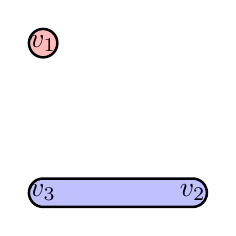
\begin{tikzpicture}[x=0.95cm,y=0.95cm]
  \fill[red!70, fill opacity=0.38] (0.000,2.000) circle[radius=0.19];
  \fill[blue!65, fill opacity=0.38] (0.000,0.190) arc[start angle=90.00, end angle=270.00, radius=0.19] -- (2.000,-0.190) arc[start angle=-90.00, end angle=90.00, radius=0.19] -- cycle;
  \draw[black, line width=0.9pt] (0.000,2.000) circle[radius=0.19];
  \draw[black, line width=0.9pt] (0.000,0.190) arc[start angle=90.00, end angle=270.00, radius=0.19] -- (2.000,-0.190) arc[start angle=-90.00, end angle=90.00, radius=0.19] -- cycle;
  \node[inner sep=0pt] at (0.000,2.000) {$v_{1}$};
  \node[inner sep=0pt] at (0.000,0.000) {$v_{3}$};
  \node[inner sep=0pt] at (2.000,0.000) {$v_{2}$};
\end{tikzpicture}
\caption{Hypergraph St\textsubscript{2}}\end{subfigure}\hfill
\begin{subfigure}{0.45\linewidth}\centering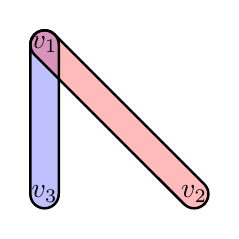
\begin{tikzpicture}[x=0.95cm,y=0.95cm]
  \fill[blue!65, fill opacity=0.38] (-0.190,0.000) arc[start angle=180.00, end angle=360.00, radius=0.19] -- (0.190,2.000) arc[start angle=0.00, end angle=180.00, radius=0.19] -- cycle;
  \fill[red!70, fill opacity=0.38] (0.134,2.134) arc[start angle=45.00, end angle=225.00, radius=0.19] -- (1.866,-0.134) arc[start angle=-135.00, end angle=45.00, radius=0.19] -- cycle;
  \draw[black, line width=0.9pt] (-0.190,0.000) arc[start angle=180.00, end angle=360.00, radius=0.19] -- (0.190,2.000) arc[start angle=0.00, end angle=180.00, radius=0.19] -- cycle;
  \draw[black, line width=0.9pt] (0.134,2.134) arc[start angle=45.00, end angle=225.00, radius=0.19] -- (1.866,-0.134) arc[start angle=-135.00, end angle=45.00, radius=0.19] -- cycle;
  \node[inner sep=0pt] at (0.000,2.000) {$v_{1}$};
  \node[inner sep=0pt] at (0.000,0.000) {$v_{3}$};
  \node[inner sep=0pt] at (2.000,0.000) {$v_{2}$};
\end{tikzpicture}
\caption{Transversal of St\textsubscript{2}}\end{subfigure}\\[8pt]
\begin{subfigure}{0.45\linewidth}\centering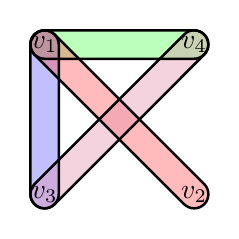
\begin{tikzpicture}[x=0.95cm,y=0.95cm]
  \fill[green!70, fill opacity=0.38] (0.000,2.190) arc[start angle=90.00, end angle=270.00, radius=0.19] -- (2.000,1.810) arc[start angle=-90.00, end angle=90.00, radius=0.19] -- cycle;
  \fill[blue!65, fill opacity=0.38] (-0.190,0.000) arc[start angle=180.00, end angle=360.00, radius=0.19] -- (0.190,2.000) arc[start angle=0.00, end angle=180.00, radius=0.19] -- cycle;
  \fill[red!70, fill opacity=0.38] (0.134,2.134) arc[start angle=45.00, end angle=225.00, radius=0.19] -- (1.866,-0.134) arc[start angle=-135.00, end angle=45.00, radius=0.19] -- cycle;
  \fill[purple!45, fill opacity=0.38] (-0.134,0.134) arc[start angle=135.00, end angle=315.00, radius=0.19] -- (2.134,1.866) arc[start angle=-45.00, end angle=135.00, radius=0.19] -- cycle;
  \draw[black, line width=0.9pt] (0.000,2.190) arc[start angle=90.00, end angle=270.00, radius=0.19] -- (2.000,1.810) arc[start angle=-90.00, end angle=90.00, radius=0.19] -- cycle;
  \draw[black, line width=0.9pt] (-0.190,0.000) arc[start angle=180.00, end angle=360.00, radius=0.19] -- (0.190,2.000) arc[start angle=0.00, end angle=180.00, radius=0.19] -- cycle;
  \draw[black, line width=0.9pt] (0.134,2.134) arc[start angle=45.00, end angle=225.00, radius=0.19] -- (1.866,-0.134) arc[start angle=-135.00, end angle=45.00, radius=0.19] -- cycle;
  \draw[black, line width=0.9pt] (-0.134,0.134) arc[start angle=135.00, end angle=315.00, radius=0.19] -- (2.134,1.866) arc[start angle=-45.00, end angle=135.00, radius=0.19] -- cycle;
  \node[inner sep=0pt] at (0.000,2.000) {$v_{1}$};
  \node[inner sep=0pt] at (2.000,2.000) {$v_{4}$};
  \node[inner sep=0pt] at (0.000,0.000) {$v_{3}$};
  \node[inner sep=0pt] at (2.000,0.000) {$v_{2}$};
\end{tikzpicture}
\caption{Hypergraph Pn\textsubscript{3}}\end{subfigure}\hfill
\begin{subfigure}{0.45\linewidth}\centering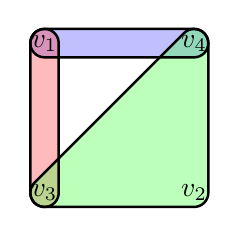
\begin{tikzpicture}[x=0.95cm,y=0.95cm]
  \fill[blue!65, fill opacity=0.38] (0.000,2.190) arc[start angle=90.00, end angle=270.00, radius=0.19] -- (2.000,1.810) arc[start angle=-90.00, end angle=90.00, radius=0.19] -- cycle;
  \fill[red!70, fill opacity=0.38] (-0.190,0.000) arc[start angle=180.00, end angle=360.00, radius=0.19] -- (0.190,2.000) arc[start angle=0.00, end angle=180.00, radius=0.19] -- cycle;
  \fill[green!70, fill opacity=0.38] (-0.134,0.134) arc[start angle=135.00, end angle=270.00, radius=0.19] -- (2.000,-0.190) arc[start angle=-90.00, end angle=0.00, radius=0.19] -- (2.190,2.000) arc[start angle=0.00, end angle=135.00, radius=0.19] -- cycle;
  \draw[black, line width=0.9pt] (0.000,2.190) arc[start angle=90.00, end angle=270.00, radius=0.19] -- (2.000,1.810) arc[start angle=-90.00, end angle=90.00, radius=0.19] -- cycle;
  \draw[black, line width=0.9pt] (-0.190,0.000) arc[start angle=180.00, end angle=360.00, radius=0.19] -- (0.190,2.000) arc[start angle=0.00, end angle=180.00, radius=0.19] -- cycle;
  \draw[black, line width=0.9pt] (-0.134,0.134) arc[start angle=135.00, end angle=270.00, radius=0.19] -- (2.000,-0.190) arc[start angle=-90.00, end angle=0.00, radius=0.19] -- (2.190,2.000) arc[start angle=0.00, end angle=135.00, radius=0.19] -- cycle;
  \node[inner sep=0pt] at (0.000,2.000) {$v_{1}$};
  \node[inner sep=0pt] at (2.000,2.000) {$v_{4}$};
  \node[inner sep=0pt] at (0.000,0.000) {$v_{3}$};
  \node[inner sep=0pt] at (2.000,0.000) {$v_{2}$};
\end{tikzpicture}
\caption{Transversal of Pn\textsubscript{3}}\end{subfigure}
\caption{Hypergraphs St\textsubscript{2} and Pn\textsubscript{3} and their transversals.}\label{fig:st2-pn3}
\end{figure}

In $\overline{Pn_3}$, the frequencies of $v_1,v_2,v_3$, and $v_4$ are $1$, $\frac{2}{3}$, $\frac{1}{2}$, and $\frac{1}{2}$, respectively. We see that all vertices of the hypergraph are above the frequency threshold of \FKA{} with $v_1$ being the most frequent. Choosing $v_1$ gives an instance of $St_2$ and $D_{1,0}$, whereas choosing $v_2$ gives instances of $D_{1,1}$ and interestingly, $D_{3,1}:\{\{v_1\},\{v_2\},\{v_3\}\},\{\{v_1,\mathbf{v_2},v_3\}\}$, and choosing $v_4$ or $v_3$ gives $St_2$ and $D_{2,1}$. While the hypergraph has the automorphism group $S_2$, decomposition can change it's automorphism group to $S_3$, giving us an instance of gaining symmetry in \FKA{} decomposition.

Lastly, in $Pn_3$, $v_1,v_4$, and $v_3$ are frequent (as defined by \FKA{} preconditions) with frequency $\frac{2}{3}$, while $v_2$ is considered infrequent and has frequency $\frac{1}{3}$ (see Figure \ref{fig:st2-pn3}). Here, removing $v_1$ gives optimal results, with an instance of $D_{1,2}$ and an instance of $D_{3,1}$. Choosing $v_2$, which is excluded by all but the most basic rule, produces the worst-case performance by instantiating $K_3$ and St\textsubscript{2}. Choosing $v_4$ or $v_3$ gives 5 nodes with St\textsubscript{2} and $D_{2,1}$.

\subsubsection*{Hypergraphs $G$ with $\Aut(G)\cong S_3$}

Up 3 vertices, hypergraphs such as $D_{1,1}$, $D_{3,1}:\{\{v_1\},\{v_2\},\{v_3\}\},\{\{v_1,\mathbf{v_2},v_3\}\}$, and $K_3:\{\{v_1,\mathbf{v_2}\},\{v_1,v_3\},\{v_2,v_3\}\}$ have automorphism groups isomorphic to $S_3$. Additionally, on 4 vertices, hypergraphs denoted
\begin{gather*}
St_3:\{\{v_1,v_2\},\{v_1,v_3\},\{v_1,v_4\}\},\{\{v_1\},\{v_2,v_3,v_4\}\},\\[4pt]
hw_3:\{\{v_1,v_4\},\{v_2,v_4\},\{v_3,v_4\},\{v_1,v_2,v_3\}\},\{\{v_1,v_4\},\{v_2,v_4\},\{v_3,v_4\},\{v_1,v_2,v_3\}\},\\[4pt]
K_3^{\cdot}:\{\{v_2\},\{v_1,v_3\},\{v_2,v_4\},\{v_3,v_4\}\},\{\{v_1,v_2,v_3,v_4\}\}.
\end{gather*}

\begin{figure}[tp]
\centering
\begin{subfigure}{0.45\linewidth}\centering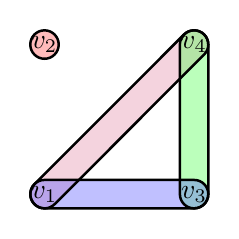
\begin{tikzpicture}[x=0.95cm,y=0.95cm]
  \fill[red!70, fill opacity=0.38] (0.000,2.000) circle[radius=0.19];
  \fill[purple!45, fill opacity=0.38] (-0.134,0.134) arc[start angle=135.00, end angle=315.00, radius=0.19] -- (2.134,1.866) arc[start angle=-45.00, end angle=135.00, radius=0.19] -- cycle;
  \fill[green!70, fill opacity=0.38] (1.810,0.000) arc[start angle=180.00, end angle=360.00, radius=0.19] -- (2.190,2.000) arc[start angle=0.00, end angle=180.00, radius=0.19] -- cycle;
  \fill[blue!65, fill opacity=0.38] (0.000,0.190) arc[start angle=90.00, end angle=270.00, radius=0.19] -- (2.000,-0.190) arc[start angle=-90.00, end angle=90.00, radius=0.19] -- cycle;
  \draw[black, line width=0.9pt] (0.000,2.000) circle[radius=0.19];
  \draw[black, line width=0.9pt] (-0.134,0.134) arc[start angle=135.00, end angle=315.00, radius=0.19] -- (2.134,1.866) arc[start angle=-45.00, end angle=135.00, radius=0.19] -- cycle;
  \draw[black, line width=0.9pt] (1.810,0.000) arc[start angle=180.00, end angle=360.00, radius=0.19] -- (2.190,2.000) arc[start angle=0.00, end angle=180.00, radius=0.19] -- cycle;
  \draw[black, line width=0.9pt] (0.000,0.190) arc[start angle=90.00, end angle=270.00, radius=0.19] -- (2.000,-0.190) arc[start angle=-90.00, end angle=90.00, radius=0.19] -- cycle;
  \node[inner sep=0pt] at (0.000,2.000) {$v_{2}$};
  \node[inner sep=0pt] at (2.000,2.000) {$v_{4}$};
  \node[inner sep=0pt] at (0.000,0.000) {$v_{1}$};
  \node[inner sep=0pt] at (2.000,0.000) {$v_{3}$};
\end{tikzpicture}
\caption{Hypergraph $K_3^{\cdot}$}\end{subfigure}\hfill
\begin{subfigure}{0.45\linewidth}\centering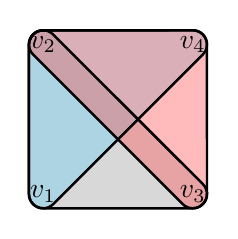
\begin{tikzpicture}[x=0.95cm,y=0.95cm]
  \fill[gray!80, fill opacity=0.38] (-0.190,0.000) arc[start angle=180.00, end angle=270.00, radius=0.19] -- (2.000,-0.190) arc[start angle=-90.00, end angle=45.00, radius=0.19] -- (0.134,2.134) arc[start angle=45.00, end angle=180.00, radius=0.19] -- cycle;
  \fill[cyan!60, fill opacity=0.38] (-0.190,0.000) arc[start angle=180.00, end angle=315.00, radius=0.19] -- (2.134,1.866) arc[start angle=-45.00, end angle=90.00, radius=0.19] -- (0.000,2.190) arc[start angle=90.00, end angle=180.00, radius=0.19] -- cycle;
  \fill[red!70, fill opacity=0.38] (0.000,2.190) arc[start angle=90.00, end angle=225.00, radius=0.19] -- (1.866,-0.134) arc[start angle=-135.00, end angle=0.00, radius=0.19] -- (2.190,2.000) arc[start angle=0.00, end angle=90.00, radius=0.19] -- cycle;
  \draw[black, line width=0.9pt] (-0.190,0.000) arc[start angle=180.00, end angle=270.00, radius=0.19] -- (2.000,-0.190) arc[start angle=-90.00, end angle=45.00, radius=0.19] -- (0.134,2.134) arc[start angle=45.00, end angle=180.00, radius=0.19] -- cycle;
  \draw[black, line width=0.9pt] (-0.190,0.000) arc[start angle=180.00, end angle=315.00, radius=0.19] -- (2.134,1.866) arc[start angle=-45.00, end angle=90.00, radius=0.19] -- (0.000,2.190) arc[start angle=90.00, end angle=180.00, radius=0.19] -- cycle;
  \draw[black, line width=0.9pt] (0.000,2.190) arc[start angle=90.00, end angle=225.00, radius=0.19] -- (1.866,-0.134) arc[start angle=-135.00, end angle=0.00, radius=0.19] -- (2.190,2.000) arc[start angle=0.00, end angle=90.00, radius=0.19] -- cycle;
  \node[inner sep=0pt] at (0.000,2.000) {$v_{2}$};
  \node[inner sep=0pt] at (2.000,2.000) {$v_{4}$};
  \node[inner sep=0pt] at (0.000,0.000) {$v_{1}$};
  \node[inner sep=0pt] at (2.000,0.000) {$v_{3}$};
\end{tikzpicture}
\caption{Transversal of $K_3^{\cdot}$}\end{subfigure}\\[8pt]
\begin{subfigure}{0.45\linewidth}\centering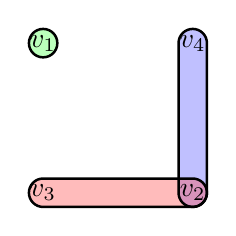
\begin{tikzpicture}[x=0.95cm,y=0.95cm]
  \fill[green!70, fill opacity=0.38] (0.000,2.000) circle[radius=0.19];
  \fill[blue!65, fill opacity=0.38] (1.810,0.000) arc[start angle=180.00, end angle=360.00, radius=0.19] -- (2.190,2.000) arc[start angle=0.00, end angle=180.00, radius=0.19] -- cycle;
  \fill[red!70, fill opacity=0.38] (0.000,0.190) arc[start angle=90.00, end angle=270.00, radius=0.19] -- (2.000,-0.190) arc[start angle=-90.00, end angle=90.00, radius=0.19] -- cycle;
  \draw[black, line width=0.9pt] (0.000,2.000) circle[radius=0.19];
  \draw[black, line width=0.9pt] (1.810,0.000) arc[start angle=180.00, end angle=360.00, radius=0.19] -- (2.190,2.000) arc[start angle=0.00, end angle=180.00, radius=0.19] -- cycle;
  \draw[black, line width=0.9pt] (0.000,0.190) arc[start angle=90.00, end angle=270.00, radius=0.19] -- (2.000,-0.190) arc[start angle=-90.00, end angle=90.00, radius=0.19] -- cycle;
  \node[inner sep=0pt] at (0.000,2.000) {$v_{1}$};
  \node[inner sep=0pt] at (2.000,2.000) {$v_{4}$};
  \node[inner sep=0pt] at (0.000,0.000) {$v_{3}$};
  \node[inner sep=0pt] at (2.000,0.000) {$v_{2}$};
\end{tikzpicture}
\caption{Hypergraph $\overline{\text{Pn}_3}$}\end{subfigure}\hfill
\begin{subfigure}{0.45\linewidth}\centering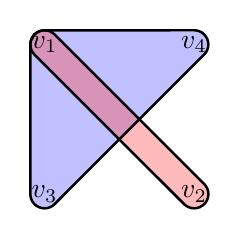
\begin{tikzpicture}[x=0.95cm,y=0.95cm]
  \fill[blue!65, fill opacity=0.38] (-0.190,0.000) arc[start angle=180.00, end angle=315.00, radius=0.19] -- (2.134,1.866) arc[start angle=-45.00, end angle=90.00, radius=0.19] -- (0.000,2.190) arc[start angle=90.00, end angle=180.00, radius=0.19] -- cycle;
  \fill[red!70, fill opacity=0.38] (0.134,2.134) arc[start angle=45.00, end angle=225.00, radius=0.19] -- (1.866,-0.134) arc[start angle=-135.00, end angle=45.00, radius=0.19] -- cycle;
  \draw[black, line width=0.9pt] (-0.190,0.000) arc[start angle=180.00, end angle=315.00, radius=0.19] -- (2.134,1.866) arc[start angle=-45.00, end angle=90.00, radius=0.19] -- (0.000,2.190) arc[start angle=90.00, end angle=180.00, radius=0.19] -- cycle;
  \draw[black, line width=0.9pt] (0.134,2.134) arc[start angle=45.00, end angle=225.00, radius=0.19] -- (1.866,-0.134) arc[start angle=-135.00, end angle=45.00, radius=0.19] -- cycle;
  \node[inner sep=0pt] at (0.000,2.000) {$v_{1}$};
  \node[inner sep=0pt] at (2.000,2.000) {$v_{4}$};
  \node[inner sep=0pt] at (0.000,0.000) {$v_{3}$};
  \node[inner sep=0pt] at (2.000,0.000) {$v_{2}$};
\end{tikzpicture}
\caption{Transversal of $\overline{\text{Pn}_3}$}\end{subfigure}
\caption{Hypergraph $K_3^{\cdot}$ and its transversal. Hypergraph $\overline{\text{Pn}_3}$ and its transversal.}\label{fig:k3dot-pn3bar}
\end{figure}

also have $S_3$ as their automorphism group.

In $St_3$, vertices $v_2$, $v_3$, and $v_4$ are frequent with frequency $\frac{1}{2}$, and $v_1$ is most frequent as it occurs in all edges (see Figure \ref{fig:d31-st3}). Removing $v_1$ results in a trivial instance of $D_{0,1}$ and $D_{3,1}$, while removing other vertices yields subhypergraphs isomorphic to $St_2$ or $D_{1,1}$. The first case results in a recursion tree with 3 nodes, whereas the latter ends up with 5 nodes.

Similarly, we see that in $hw_3$ (see Figure \ref{fig:p4-hw3}), $v_1$, $v_2$, and $v_3$ are frequent with frequency $\frac{1}{2}$ (\emph{frequent} in the context of multiple vertices having the same frequency and there existing a separate most frequent vertex) and $v_4$ is most frequent with frequency $\frac{3}{4}$ . Recursing on $v_4$ results in an instance of $D_{1,3}$, and an instance of $D_{3,1}$, thus the recursion tree of our modified implementation has 3 nodes. Choosing any other vertex leads to two instances of $St_2$, which has 3 nodes. So, the maximum size of the recursion tree is 7 nodes.

The hypergraph $K_3^{\cdot}$ is defined as a cycle $C_3$ together with a singleton vertex (see Figure \ref{fig:k3dot-pn3bar}). The vertex $v_2$ is most frequent with frequency 1, and the other vertices are frequent with a frequency of $\frac{2}{3}$. Removing $v_2$ gives $D_{0,1}$ and $K_3$ for a recursion tree with 5 nodes. Choosing any of the other vertices gives instances of $D_{1,3}$ and $St_2$, which again, results in a tree with 5 nodes.

Lastly, $K_3$ is invariant under any permutation and in general $\Aut(K_n)\cong S_n$ (see Figure \ref{fig:k3-k4minus}). Selecting $v_1$ as the splitting vertex, we get two cases of $D_{1,2}$, which are trivial due to our modifications, and once again we have a tree of size 3. Another interesting observation is that both $K_3$ and $hw_3$ are also self-transversal hypergraphs. In fact, the next well-known self-transversal hypergraph is on 7 vertices, namely the fano plane hypergraph, which is identified as a difficult case for \FKA.

\begin{figure}[tp]
\centering
\begin{subfigure}{0.45\linewidth}\centering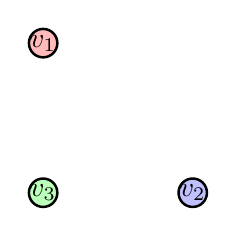
\begin{tikzpicture}[x=0.95cm,y=0.95cm]
  \fill[red!70, fill opacity=0.38] (0.000,2.000) circle[radius=0.19];
  \fill[green!70, fill opacity=0.38] (0.000,0.000) circle[radius=0.19];
  \fill[blue!65, fill opacity=0.38] (2.000,0.000) circle[radius=0.19];
  \draw[black, line width=0.9pt] (0.000,2.000) circle[radius=0.19];
  \draw[black, line width=0.9pt] (0.000,0.000) circle[radius=0.19];
  \draw[black, line width=0.9pt] (2.000,0.000) circle[radius=0.19];
  \node[inner sep=0pt] at (0.000,2.000) {$v_{1}$};
  \node[inner sep=0pt] at (0.000,0.000) {$v_{3}$};
  \node[inner sep=0pt] at (2.000,0.000) {$v_{2}$};
\end{tikzpicture}
\caption{Hypergraph $D_{3,1}$}\end{subfigure}\hfill
\begin{subfigure}{0.45\linewidth}\centering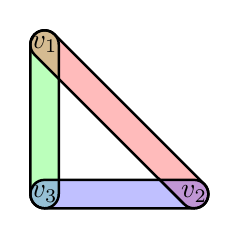
\begin{tikzpicture}[x=0.95cm,y=0.95cm]
  \fill[green!70, fill opacity=0.38] (-0.190,0.000) arc[start angle=180.00, end angle=360.00, radius=0.19] -- (0.190,2.000) arc[start angle=0.00, end angle=180.00, radius=0.19] -- cycle;
  \fill[red!70, fill opacity=0.38] (0.134,2.134) arc[start angle=45.00, end angle=225.00, radius=0.19] -- (1.866,-0.134) arc[start angle=-135.00, end angle=45.00, radius=0.19] -- cycle;
  \fill[blue!65, fill opacity=0.38] (0.000,0.190) arc[start angle=90.00, end angle=270.00, radius=0.19] -- (2.000,-0.190) arc[start angle=-90.00, end angle=90.00, radius=0.19] -- cycle;
  \draw[black, line width=0.9pt] (-0.190,0.000) arc[start angle=180.00, end angle=360.00, radius=0.19] -- (0.190,2.000) arc[start angle=0.00, end angle=180.00, radius=0.19] -- cycle;
  \draw[black, line width=0.9pt] (0.134,2.134) arc[start angle=45.00, end angle=225.00, radius=0.19] -- (1.866,-0.134) arc[start angle=-135.00, end angle=45.00, radius=0.19] -- cycle;
  \draw[black, line width=0.9pt] (0.000,0.190) arc[start angle=90.00, end angle=270.00, radius=0.19] -- (2.000,-0.190) arc[start angle=-90.00, end angle=90.00, radius=0.19] -- cycle;
  \node[inner sep=0pt] at (0.000,2.000) {$v_{1}$};
  \node[inner sep=0pt] at (0.000,0.000) {$v_{3}$};
  \node[inner sep=0pt] at (2.000,0.000) {$v_{2}$};
\end{tikzpicture}
\caption{Transversal of $D_{3,1}$}\end{subfigure}\\[8pt]
\begin{subfigure}{0.45\linewidth}\centering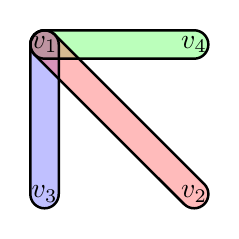
\begin{tikzpicture}[x=0.95cm,y=0.95cm]
  \fill[green!70, fill opacity=0.38] (0.000,2.190) arc[start angle=90.00, end angle=270.00, radius=0.19] -- (2.000,1.810) arc[start angle=-90.00, end angle=90.00, radius=0.19] -- cycle;
  \fill[blue!65, fill opacity=0.38] (-0.190,0.000) arc[start angle=180.00, end angle=360.00, radius=0.19] -- (0.190,2.000) arc[start angle=0.00, end angle=180.00, radius=0.19] -- cycle;
  \fill[red!70, fill opacity=0.38] (0.134,2.134) arc[start angle=45.00, end angle=225.00, radius=0.19] -- (1.866,-0.134) arc[start angle=-135.00, end angle=45.00, radius=0.19] -- cycle;
  \draw[black, line width=0.9pt] (0.000,2.190) arc[start angle=90.00, end angle=270.00, radius=0.19] -- (2.000,1.810) arc[start angle=-90.00, end angle=90.00, radius=0.19] -- cycle;
  \draw[black, line width=0.9pt] (-0.190,0.000) arc[start angle=180.00, end angle=360.00, radius=0.19] -- (0.190,2.000) arc[start angle=0.00, end angle=180.00, radius=0.19] -- cycle;
  \draw[black, line width=0.9pt] (0.134,2.134) arc[start angle=45.00, end angle=225.00, radius=0.19] -- (1.866,-0.134) arc[start angle=-135.00, end angle=45.00, radius=0.19] -- cycle;
  \node[inner sep=0pt] at (0.000,2.000) {$v_{1}$};
  \node[inner sep=0pt] at (2.000,2.000) {$v_{4}$};
  \node[inner sep=0pt] at (0.000,0.000) {$v_{3}$};
  \node[inner sep=0pt] at (2.000,0.000) {$v_{2}$};
\end{tikzpicture}
\caption{Hypergraph St\textsubscript{3}}\end{subfigure}\hfill
\begin{subfigure}{0.45\linewidth}\centering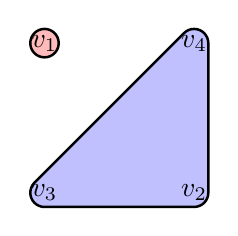
\begin{tikzpicture}[x=0.95cm,y=0.95cm]
  \fill[red!70, fill opacity=0.38] (0.000,2.000) circle[radius=0.19];
  \fill[blue!65, fill opacity=0.38] (-0.134,0.134) arc[start angle=135.00, end angle=270.00, radius=0.19] -- (2.000,-0.190) arc[start angle=-90.00, end angle=0.00, radius=0.19] -- (2.190,2.000) arc[start angle=0.00, end angle=135.00, radius=0.19] -- cycle;
  \draw[black, line width=0.9pt] (0.000,2.000) circle[radius=0.19];
  \draw[black, line width=0.9pt] (-0.134,0.134) arc[start angle=135.00, end angle=270.00, radius=0.19] -- (2.000,-0.190) arc[start angle=-90.00, end angle=0.00, radius=0.19] -- (2.190,2.000) arc[start angle=0.00, end angle=135.00, radius=0.19] -- cycle;
  \node[inner sep=0pt] at (0.000,2.000) {$v_{1}$};
  \node[inner sep=0pt] at (2.000,2.000) {$v_{4}$};
  \node[inner sep=0pt] at (0.000,0.000) {$v_{3}$};
  \node[inner sep=0pt] at (2.000,0.000) {$v_{2}$};
\end{tikzpicture}
\caption{Transversal of St\textsubscript{3}}\end{subfigure}
\caption{Hypergraph $D_{3,1}$ and its transversal. Hypergraph St\textsubscript{3} and its transversal.}\label{fig:d31-st3}
\end{figure}

\subsubsection*{Hypergraphs $G$ with $\Aut(G)\cong S_2\times S_2$}

Hypergraphs on 4 vertices with automorphism group isomorphic to $S_2\times S_2$ are denoted as $D_{2,1}$,
\[
K_4^-:\{\{v_3,v_4\},\{v_1,v_4\},\{v_1,v_3\},\{v_2,v_4\},\{v_2,v_3\}\},\{\{v_1,v_2,v_3,v_4\},\{v_1,v_2,v_4\},\{v_1,v_3,v_4\}\},
\]
\[
K_2^{\cdot\cdot}:\{\{v_1,v_2\},\{v_3,v_4\}\},\{\{v_1,v_2\},\{v_3,v_4\}\}.
\]
The symmetry of hypergraphs $K_2^{\cdot\cdot}$ and $K_4^-$ is generated by permutations like $\langle(v_1,v_2),(v_3,v_4)\rangle$, i.e., we can either permute $(v_1,v_2)$ or $(v_3,v_4)$ or both.

$K_4^-$ is a complete graph on 4 vertices missing one edge, where all vertices have maximum frequency $\frac{2}{3}$ (see Figure \ref{fig:k3-k4minus}). Recursing on any vertex leads to hypergraphs such as $K_3$ and $D_{2,1}$, resulting in a recursion tree with 5 nodes.

$K_2^{\cdot\cdot}$ is the complete graph $K_2$ with two singleton vertices, with its transversal hypergraph having 2 edges each containing 3 vertices (see Figure \ref{fig:k2dd-c4}). $v_1$ and $v_2$ are most frequent with frequency 1, and $v_3$ and $v_4$ are frequent with frequency $\frac{1}{2}$. Choosing $v_3$ or $v_4$ gives an instance of $D_{3,1}$ and $D_{2,1}$, which results in 3 nodes in the recursion tree, while choosing $v_1$ or $v_2$ gives rise to $St_2$ and $D_{1,0}$, for a total of 5 nodes. Interestingly, in this case, choosing the vertex with the highest frequency is not optimal in terms of tree size.

\subsubsection*{Hypergraphs $G$ with $\Aut(G)\cong D_4$}

The cycle graph $C_4:\{\{v_1,v_3\},\{v_2,v_3\},\{v_2,v_4\},\{v_1,v_2\}\},\{\{v_1,v_2\},\{v_2,v_3\},\{v_3,v_4\}\}$ is invariant under both rotation and reflection, leading to the automorphism group $D_4$ (see Figure \ref{fig:k2dd-c4}). All vertices in $C_4$ are frequent, with no distinct most frequent vertex. Like $K_n$, each vertex is isomorphic, implying that removing any vertex gives isomorphic hypergraphs. Choosing any vertex produces an instance of $St_2$ and an instance of $D_{2,1}$, totaling five nodes in the tree.

\begin{figure}[tp]
\centering
\begin{subfigure}{0.45\linewidth}\centering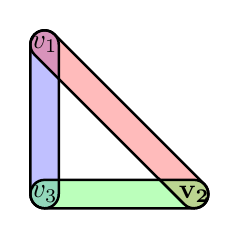
\begin{tikzpicture}[x=0.95cm,y=0.95cm]
  \fill[blue!65, fill opacity=0.38] (-0.190,0.000) arc[start angle=180.00, end angle=360.00, radius=0.19] -- (0.190,2.000) arc[start angle=0.00, end angle=180.00, radius=0.19] -- cycle;
  \fill[red!70, fill opacity=0.38] (0.134,2.134) arc[start angle=45.00, end angle=225.00, radius=0.19] -- (1.866,-0.134) arc[start angle=-135.00, end angle=45.00, radius=0.19] -- cycle;
  \fill[green!70, fill opacity=0.38] (0.000,0.190) arc[start angle=90.00, end angle=270.00, radius=0.19] -- (2.000,-0.190) arc[start angle=-90.00, end angle=90.00, radius=0.19] -- cycle;
  \draw[black, line width=0.9pt] (-0.190,0.000) arc[start angle=180.00, end angle=360.00, radius=0.19] -- (0.190,2.000) arc[start angle=0.00, end angle=180.00, radius=0.19] -- cycle;
  \draw[black, line width=0.9pt] (0.134,2.134) arc[start angle=45.00, end angle=225.00, radius=0.19] -- (1.866,-0.134) arc[start angle=-135.00, end angle=45.00, radius=0.19] -- cycle;
  \draw[black, line width=0.9pt] (0.000,0.190) arc[start angle=90.00, end angle=270.00, radius=0.19] -- (2.000,-0.190) arc[start angle=-90.00, end angle=90.00, radius=0.19] -- cycle;
  \node[inner sep=0pt] at (0.000,2.000) {$v_{1}$};
  \node[inner sep=0pt] at (0.000,0.000) {$v_{3}$};
  \node[inner sep=0pt] at (2.000,0.000) {$\mathbf{v_{2}}$};
\end{tikzpicture}
\caption{Hypergraph $K_3$}\end{subfigure}\hfill
\begin{subfigure}{0.45\linewidth}\centering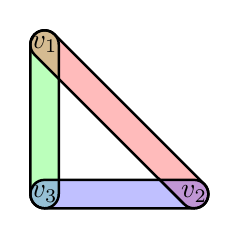
\begin{tikzpicture}[x=0.95cm,y=0.95cm]
  \fill[green!70, fill opacity=0.38] (-0.190,0.000) arc[start angle=180.00, end angle=360.00, radius=0.19] -- (0.190,2.000) arc[start angle=0.00, end angle=180.00, radius=0.19] -- cycle;
  \fill[red!70, fill opacity=0.38] (0.134,2.134) arc[start angle=45.00, end angle=225.00, radius=0.19] -- (1.866,-0.134) arc[start angle=-135.00, end angle=45.00, radius=0.19] -- cycle;
  \fill[blue!65, fill opacity=0.38] (0.000,0.190) arc[start angle=90.00, end angle=270.00, radius=0.19] -- (2.000,-0.190) arc[start angle=-90.00, end angle=90.00, radius=0.19] -- cycle;
  \draw[black, line width=0.9pt] (-0.190,0.000) arc[start angle=180.00, end angle=360.00, radius=0.19] -- (0.190,2.000) arc[start angle=0.00, end angle=180.00, radius=0.19] -- cycle;
  \draw[black, line width=0.9pt] (0.134,2.134) arc[start angle=45.00, end angle=225.00, radius=0.19] -- (1.866,-0.134) arc[start angle=-135.00, end angle=45.00, radius=0.19] -- cycle;
  \draw[black, line width=0.9pt] (0.000,0.190) arc[start angle=90.00, end angle=270.00, radius=0.19] -- (2.000,-0.190) arc[start angle=-90.00, end angle=90.00, radius=0.19] -- cycle;
  \node[inner sep=0pt] at (0.000,2.000) {$v_{1}$};
  \node[inner sep=0pt] at (0.000,0.000) {$v_{3}$};
  \node[inner sep=0pt] at (2.000,0.000) {$v_{2}$};
\end{tikzpicture}
\caption{Transversal of $K_3$}\end{subfigure}\\[8pt]
\begin{subfigure}{0.45\linewidth}\centering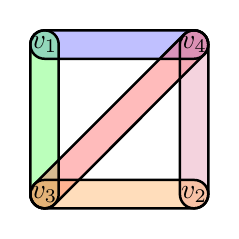
\begin{tikzpicture}[x=0.95cm,y=0.95cm]
  \fill[blue!65, fill opacity=0.38] (0.000,2.190) arc[start angle=90.00, end angle=270.00, radius=0.19] -- (2.000,1.810) arc[start angle=-90.00, end angle=90.00, radius=0.19] -- cycle;
  \fill[green!70, fill opacity=0.38] (-0.190,0.000) arc[start angle=180.00, end angle=360.00, radius=0.19] -- (0.190,2.000) arc[start angle=0.00, end angle=180.00, radius=0.19] -- cycle;
  \fill[red!70, fill opacity=0.38] (-0.134,0.134) arc[start angle=135.00, end angle=315.00, radius=0.19] -- (2.134,1.866) arc[start angle=-45.00, end angle=135.00, radius=0.19] -- cycle;
  \fill[purple!45, fill opacity=0.38] (1.810,0.000) arc[start angle=180.00, end angle=360.00, radius=0.19] -- (2.190,2.000) arc[start angle=0.00, end angle=180.00, radius=0.19] -- cycle;
  \fill[orange!70, fill opacity=0.38] (0.000,0.190) arc[start angle=90.00, end angle=270.00, radius=0.19] -- (2.000,-0.190) arc[start angle=-90.00, end angle=90.00, radius=0.19] -- cycle;
  \draw[black, line width=0.9pt] (0.000,2.190) arc[start angle=90.00, end angle=270.00, radius=0.19] -- (2.000,1.810) arc[start angle=-90.00, end angle=90.00, radius=0.19] -- cycle;
  \draw[black, line width=0.9pt] (-0.190,0.000) arc[start angle=180.00, end angle=360.00, radius=0.19] -- (0.190,2.000) arc[start angle=0.00, end angle=180.00, radius=0.19] -- cycle;
  \draw[black, line width=0.9pt] (-0.134,0.134) arc[start angle=135.00, end angle=315.00, radius=0.19] -- (2.134,1.866) arc[start angle=-45.00, end angle=135.00, radius=0.19] -- cycle;
  \draw[black, line width=0.9pt] (1.810,0.000) arc[start angle=180.00, end angle=360.00, radius=0.19] -- (2.190,2.000) arc[start angle=0.00, end angle=180.00, radius=0.19] -- cycle;
  \draw[black, line width=0.9pt] (0.000,0.190) arc[start angle=90.00, end angle=270.00, radius=0.19] -- (2.000,-0.190) arc[start angle=-90.00, end angle=90.00, radius=0.19] -- cycle;
  \node[inner sep=0pt] at (0.000,2.000) {$v_{1}$};
  \node[inner sep=0pt] at (2.000,2.000) {$v_{4}$};
  \node[inner sep=0pt] at (0.000,0.000) {$v_{3}$};
  \node[inner sep=0pt] at (2.000,0.000) {$v_{2}$};
\end{tikzpicture}
\caption{Hypergraph $K_4^-$}\end{subfigure}\hfill
\begin{subfigure}{0.45\linewidth}\centering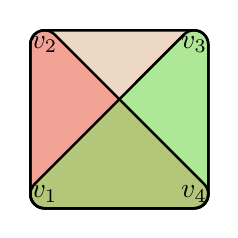
\begin{tikzpicture}[x=0.95cm,y=0.95cm]
  \fill[brown!80, fill opacity=0.38] (-0.190,0.000) arc[start angle=180.00, end angle=270.00, radius=0.19] -- (2.000,-0.190) arc[start angle=-90.00, end angle=0.00, radius=0.19] -- (2.190,2.000) arc[start angle=0.00, end angle=90.00, radius=0.19] -- (0.000,2.190) arc[start angle=90.00, end angle=180.00, radius=0.19] -- cycle;
  \fill[red!70, fill opacity=0.38] (-0.190,0.000) arc[start angle=180.00, end angle=270.00, radius=0.19] -- (2.000,-0.190) arc[start angle=-90.00, end angle=45.00, radius=0.19] -- (0.134,2.134) arc[start angle=45.00, end angle=180.00, radius=0.19] -- cycle;
  \fill[green!70, fill opacity=0.38] (-0.134,0.134) arc[start angle=135.00, end angle=270.00, radius=0.19] -- (2.000,-0.190) arc[start angle=-90.00, end angle=0.00, radius=0.19] -- (2.190,2.000) arc[start angle=0.00, end angle=135.00, radius=0.19] -- cycle;
  \draw[black, line width=0.9pt] (-0.190,0.000) arc[start angle=180.00, end angle=270.00, radius=0.19] -- (2.000,-0.190) arc[start angle=-90.00, end angle=0.00, radius=0.19] -- (2.190,2.000) arc[start angle=0.00, end angle=90.00, radius=0.19] -- (0.000,2.190) arc[start angle=90.00, end angle=180.00, radius=0.19] -- cycle;
  \draw[black, line width=0.9pt] (-0.190,0.000) arc[start angle=180.00, end angle=270.00, radius=0.19] -- (2.000,-0.190) arc[start angle=-90.00, end angle=45.00, radius=0.19] -- (0.134,2.134) arc[start angle=45.00, end angle=180.00, radius=0.19] -- cycle;
  \draw[black, line width=0.9pt] (-0.134,0.134) arc[start angle=135.00, end angle=270.00, radius=0.19] -- (2.000,-0.190) arc[start angle=-90.00, end angle=0.00, radius=0.19] -- (2.190,2.000) arc[start angle=0.00, end angle=135.00, radius=0.19] -- cycle;
  \node[inner sep=0pt] at (0.000,2.000) {$v_{2}$};
  \node[inner sep=0pt] at (2.000,2.000) {$v_{3}$};
  \node[inner sep=0pt] at (0.000,0.000) {$v_{1}$};
  \node[inner sep=0pt] at (2.000,0.000) {$v_{4}$};
\end{tikzpicture}
\caption{Transversal of $K_4^-$}\end{subfigure}
\caption{Hypergraph $K_3$ and its transversal. Hypergraph $K_4^-$ and its transversal.}\label{fig:k3-k4minus}
\end{figure}

\subsubsection*{Hypergraphs $G$ with $\Aut(G)\cong S_4$}

The hypergraphs
\[
D_{4,1}:\{\{v_1\},\{v_2\},\{v_3\},\{v_4\}\},\{\{\mathbf{v_1},\mathbf{v_2},\mathbf{v_3},\mathbf{v_4}\}\},
\]
\[
K_4:\{\{v_1,v_2\},\{v_2,v_3\},\{v_2,v_4\},\{v_1,v_3\},\{v_3,v_4\},\{v_1,v_4\}\},\{\{v_1,v_2,v_3,v_4\},\{v_1,v_2,v_4,v_3\},\{v_1,v_3,v_2,v_4\}\}.
\]
and $D_{1,0}$ are invariant under any permutation. Consequently, their automorphism group is isomorphic to $S_4$.

Specifically, $K_4$ has complete symmetry with respect to permutations, and all vertices have frequency $\frac{3}{4}$. Therefore, choosing any splitting vertex during recursion results in two instances of $K_3$ and $D_{3,1}$, yielding a recursion tree with five nodes.

Altogether, up to 4 vertices, there are 13 pairs of distinct hypergraphs, for a total of 30 equivalence classes i.e. distinct hypergraphs under permutation (see Table 3.1). There are in total 168 distinct hypergraphs on 4 vertices (see Table 3.2), which are all permutations of the abovementioned structures. By elementary group theory, the number of different permutations of these hypergraphs is $\frac{24}{|G|}$, where $G$ is the automorphism group of the given hypergraph. There are $\binom{4}{k}$ permutations for $D_{k,1}$, $\binom{4}{3}\cdot 4=12$ permutations for $St_2$, and 4 permutations for $St_3$ and $hw_3$. Similarly, there are $\binom{4}{3}$ permutations for $K_3$, 6 for $K_4^-$,

\begin{figure}[tp]
\centering
\begin{subfigure}{0.45\linewidth}\centering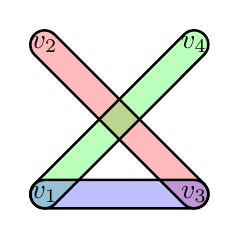
\begin{tikzpicture}[x=0.95cm,y=0.95cm]
  \fill[red!70, fill opacity=0.38] (0.134,2.134) arc[start angle=45.00, end angle=225.00, radius=0.19] -- (1.866,-0.134) arc[start angle=-135.00, end angle=45.00, radius=0.19] -- cycle;
  \fill[green!70, fill opacity=0.38] (-0.134,0.134) arc[start angle=135.00, end angle=315.00, radius=0.19] -- (2.134,1.866) arc[start angle=-45.00, end angle=135.00, radius=0.19] -- cycle;
  \fill[blue!65, fill opacity=0.38] (0.000,0.190) arc[start angle=90.00, end angle=270.00, radius=0.19] -- (2.000,-0.190) arc[start angle=-90.00, end angle=90.00, radius=0.19] -- cycle;
  \draw[black, line width=0.9pt] (0.134,2.134) arc[start angle=45.00, end angle=225.00, radius=0.19] -- (1.866,-0.134) arc[start angle=-135.00, end angle=45.00, radius=0.19] -- cycle;
  \draw[black, line width=0.9pt] (-0.134,0.134) arc[start angle=135.00, end angle=315.00, radius=0.19] -- (2.134,1.866) arc[start angle=-45.00, end angle=135.00, radius=0.19] -- cycle;
  \draw[black, line width=0.9pt] (0.000,0.190) arc[start angle=90.00, end angle=270.00, radius=0.19] -- (2.000,-0.190) arc[start angle=-90.00, end angle=90.00, radius=0.19] -- cycle;
  \node[inner sep=0pt] at (0.000,2.000) {$v_{2}$};
  \node[inner sep=0pt] at (2.000,2.000) {$v_{4}$};
  \node[inner sep=0pt] at (0.000,0.000) {$v_{1}$};
  \node[inner sep=0pt] at (2.000,0.000) {$v_{3}$};
\end{tikzpicture}
\caption{Hypergraph $P_4$}\end{subfigure}\hfill
\begin{subfigure}{0.45\linewidth}\centering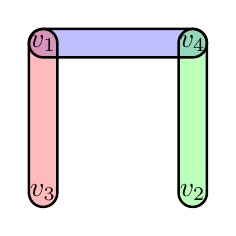
\begin{tikzpicture}[x=0.95cm,y=0.95cm]
  \fill[blue!65, fill opacity=0.38] (0.000,2.190) arc[start angle=90.00, end angle=270.00, radius=0.19] -- (2.000,1.810) arc[start angle=-90.00, end angle=90.00, radius=0.19] -- cycle;
  \fill[red!70, fill opacity=0.38] (-0.190,0.000) arc[start angle=180.00, end angle=360.00, radius=0.19] -- (0.190,2.000) arc[start angle=0.00, end angle=180.00, radius=0.19] -- cycle;
  \fill[green!70, fill opacity=0.38] (1.810,0.000) arc[start angle=180.00, end angle=360.00, radius=0.19] -- (2.190,2.000) arc[start angle=0.00, end angle=180.00, radius=0.19] -- cycle;
  \draw[black, line width=0.9pt] (0.000,2.190) arc[start angle=90.00, end angle=270.00, radius=0.19] -- (2.000,1.810) arc[start angle=-90.00, end angle=90.00, radius=0.19] -- cycle;
  \draw[black, line width=0.9pt] (-0.190,0.000) arc[start angle=180.00, end angle=360.00, radius=0.19] -- (0.190,2.000) arc[start angle=0.00, end angle=180.00, radius=0.19] -- cycle;
  \draw[black, line width=0.9pt] (1.810,0.000) arc[start angle=180.00, end angle=360.00, radius=0.19] -- (2.190,2.000) arc[start angle=0.00, end angle=180.00, radius=0.19] -- cycle;
  \node[inner sep=0pt] at (0.000,2.000) {$v_{1}$};
  \node[inner sep=0pt] at (2.000,2.000) {$v_{4}$};
  \node[inner sep=0pt] at (0.000,0.000) {$v_{3}$};
  \node[inner sep=0pt] at (2.000,0.000) {$v_{2}$};
\end{tikzpicture}
\caption{Transversal of $P_4$}\end{subfigure}\\[8pt]
\begin{subfigure}{0.45\linewidth}\centering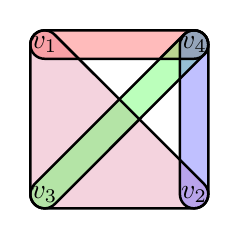
\begin{tikzpicture}[x=0.95cm,y=0.95cm]
  \fill[purple!45, fill opacity=0.38] (-0.190,0.000) arc[start angle=180.00, end angle=270.00, radius=0.19] -- (2.000,-0.190) arc[start angle=-90.00, end angle=45.00, radius=0.19] -- (0.134,2.134) arc[start angle=45.00, end angle=180.00, radius=0.19] -- cycle;
  \fill[red!70, fill opacity=0.38] (0.000,2.190) arc[start angle=90.00, end angle=270.00, radius=0.19] -- (2.000,1.810) arc[start angle=-90.00, end angle=90.00, radius=0.19] -- cycle;
  \fill[green!70, fill opacity=0.38] (-0.134,0.134) arc[start angle=135.00, end angle=315.00, radius=0.19] -- (2.134,1.866) arc[start angle=-45.00, end angle=135.00, radius=0.19] -- cycle;
  \fill[blue!65, fill opacity=0.38] (1.810,0.000) arc[start angle=180.00, end angle=360.00, radius=0.19] -- (2.190,2.000) arc[start angle=0.00, end angle=180.00, radius=0.19] -- cycle;
  \draw[black, line width=0.9pt] (-0.190,0.000) arc[start angle=180.00, end angle=270.00, radius=0.19] -- (2.000,-0.190) arc[start angle=-90.00, end angle=45.00, radius=0.19] -- (0.134,2.134) arc[start angle=45.00, end angle=180.00, radius=0.19] -- cycle;
  \draw[black, line width=0.9pt] (0.000,2.190) arc[start angle=90.00, end angle=270.00, radius=0.19] -- (2.000,1.810) arc[start angle=-90.00, end angle=90.00, radius=0.19] -- cycle;
  \draw[black, line width=0.9pt] (-0.134,0.134) arc[start angle=135.00, end angle=315.00, radius=0.19] -- (2.134,1.866) arc[start angle=-45.00, end angle=135.00, radius=0.19] -- cycle;
  \draw[black, line width=0.9pt] (1.810,0.000) arc[start angle=180.00, end angle=360.00, radius=0.19] -- (2.190,2.000) arc[start angle=0.00, end angle=180.00, radius=0.19] -- cycle;
  \node[inner sep=0pt] at (0.000,2.000) {$v_{1}$};
  \node[inner sep=0pt] at (2.000,2.000) {$v_{4}$};
  \node[inner sep=0pt] at (0.000,0.000) {$v_{3}$};
  \node[inner sep=0pt] at (2.000,0.000) {$v_{2}$};
\end{tikzpicture}
\caption{Hypergraph hw\textsubscript{3}}\end{subfigure}\hfill
\begin{subfigure}{0.45\linewidth}\centering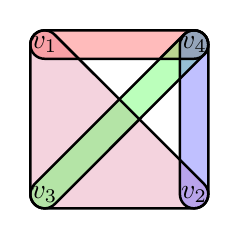
\begin{tikzpicture}[x=0.95cm,y=0.95cm]
  \fill[purple!45, fill opacity=0.38] (-0.190,0.000) arc[start angle=180.00, end angle=270.00, radius=0.19] -- (2.000,-0.190) arc[start angle=-90.00, end angle=45.00, radius=0.19] -- (0.134,2.134) arc[start angle=45.00, end angle=180.00, radius=0.19] -- cycle;
  \fill[red!70, fill opacity=0.38] (0.000,2.190) arc[start angle=90.00, end angle=270.00, radius=0.19] -- (2.000,1.810) arc[start angle=-90.00, end angle=90.00, radius=0.19] -- cycle;
  \fill[green!70, fill opacity=0.38] (-0.134,0.134) arc[start angle=135.00, end angle=315.00, radius=0.19] -- (2.134,1.866) arc[start angle=-45.00, end angle=135.00, radius=0.19] -- cycle;
  \fill[blue!65, fill opacity=0.38] (1.810,0.000) arc[start angle=180.00, end angle=360.00, radius=0.19] -- (2.190,2.000) arc[start angle=0.00, end angle=180.00, radius=0.19] -- cycle;
  \draw[black, line width=0.9pt] (-0.190,0.000) arc[start angle=180.00, end angle=270.00, radius=0.19] -- (2.000,-0.190) arc[start angle=-90.00, end angle=45.00, radius=0.19] -- (0.134,2.134) arc[start angle=45.00, end angle=180.00, radius=0.19] -- cycle;
  \draw[black, line width=0.9pt] (0.000,2.190) arc[start angle=90.00, end angle=270.00, radius=0.19] -- (2.000,1.810) arc[start angle=-90.00, end angle=90.00, radius=0.19] -- cycle;
  \draw[black, line width=0.9pt] (-0.134,0.134) arc[start angle=135.00, end angle=315.00, radius=0.19] -- (2.134,1.866) arc[start angle=-45.00, end angle=135.00, radius=0.19] -- cycle;
  \draw[black, line width=0.9pt] (1.810,0.000) arc[start angle=180.00, end angle=360.00, radius=0.19] -- (2.190,2.000) arc[start angle=0.00, end angle=180.00, radius=0.19] -- cycle;
  \node[inner sep=0pt] at (0.000,2.000) {$v_{1}$};
  \node[inner sep=0pt] at (2.000,2.000) {$v_{4}$};
  \node[inner sep=0pt] at (0.000,0.000) {$v_{3}$};
  \node[inner sep=0pt] at (2.000,0.000) {$v_{2}$};
\end{tikzpicture}
\caption{Transversal of hw\textsubscript{3}}\end{subfigure}
\caption{Hypergraph $P_4$ and its transversal. Hypergraph hw\textsubscript{3} and its transversal.}\label{fig:p4-hw3}
\end{figure}

\noindent and 1 permutation for $K_4$. The cycle $C_4$ has 3 permutations and $K_2^{\cdot\cdot}$ also has 6, while $K_3^{\cdot}$ has 4 permutations. $P_4$ has 12 permutations. Finally, $Pn_3$ and $\overline{Pn_3}$ are complementary graphs and both have 12 permutations. Adding these numbers up and taking note of self-transversal cases indeed gives us the 168 distinct hypergraphs.

The hypergraphs according to these symmetry groups are grouped in the following table:

\begin{table}[h]
\centering
\begin{tabular}{|c|c|}
\hline
$D_{4,1},K_4,D_{1,0}$ & $S_4$\\\hline
$C_4$ & $D_4$\\\hline
$D_{1,1},D_{3,1},\text{star}_3,hw_3,K_3,K_3^{\cdot}$ & $S_3$\\\hline
$D_{2,1},K_4^-,K_2^{\cdot\cdot}$ & $S_2\times S_2$\\\hline
$\text{star}_2,\text{pan}_3,\text{pan}_3',\text{path}_4$ & $S_2$\\\hline
\end{tabular}
\caption{Hypergraphs grouped by their automorphism groups.}
\end{table}

\begin{figure}[tp]
\centering
\begin{subfigure}{0.45\linewidth}\centering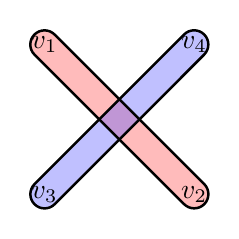
\begin{tikzpicture}[x=0.95cm,y=0.95cm]
  \fill[red!70, fill opacity=0.38] (0.134,2.134) arc[start angle=45.00, end angle=225.00, radius=0.19] -- (1.866,-0.134) arc[start angle=-135.00, end angle=45.00, radius=0.19] -- cycle;
  \fill[blue!65, fill opacity=0.38] (-0.134,0.134) arc[start angle=135.00, end angle=315.00, radius=0.19] -- (2.134,1.866) arc[start angle=-45.00, end angle=135.00, radius=0.19] -- cycle;
  \draw[black, line width=0.9pt] (0.134,2.134) arc[start angle=45.00, end angle=225.00, radius=0.19] -- (1.866,-0.134) arc[start angle=-135.00, end angle=45.00, radius=0.19] -- cycle;
  \draw[black, line width=0.9pt] (-0.134,0.134) arc[start angle=135.00, end angle=315.00, radius=0.19] -- (2.134,1.866) arc[start angle=-45.00, end angle=135.00, radius=0.19] -- cycle;
  \node[inner sep=0pt] at (0.000,2.000) {$v_{1}$};
  \node[inner sep=0pt] at (2.000,2.000) {$v_{4}$};
  \node[inner sep=0pt] at (0.000,0.000) {$v_{3}$};
  \node[inner sep=0pt] at (2.000,0.000) {$v_{2}$};
\end{tikzpicture}
\caption{Hypergraph $K_2^{\cdot\cdot}$}\end{subfigure}\hfill
\begin{subfigure}{0.45\linewidth}\centering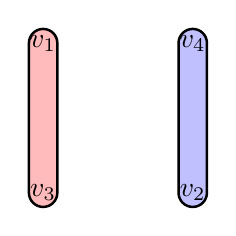
\begin{tikzpicture}[x=0.95cm,y=0.95cm]
  \fill[red!70, fill opacity=0.38] (-0.190,0.000) arc[start angle=180.00, end angle=360.00, radius=0.19] -- (0.190,2.000) arc[start angle=0.00, end angle=180.00, radius=0.19] -- cycle;
  \fill[blue!65, fill opacity=0.38] (1.810,0.000) arc[start angle=180.00, end angle=360.00, radius=0.19] -- (2.190,2.000) arc[start angle=0.00, end angle=180.00, radius=0.19] -- cycle;
  \draw[black, line width=0.9pt] (-0.190,0.000) arc[start angle=180.00, end angle=360.00, radius=0.19] -- (0.190,2.000) arc[start angle=0.00, end angle=180.00, radius=0.19] -- cycle;
  \draw[black, line width=0.9pt] (1.810,0.000) arc[start angle=180.00, end angle=360.00, radius=0.19] -- (2.190,2.000) arc[start angle=0.00, end angle=180.00, radius=0.19] -- cycle;
  \node[inner sep=0pt] at (0.000,2.000) {$v_{1}$};
  \node[inner sep=0pt] at (2.000,2.000) {$v_{4}$};
  \node[inner sep=0pt] at (0.000,0.000) {$v_{3}$};
  \node[inner sep=0pt] at (2.000,0.000) {$v_{2}$};
\end{tikzpicture}
\caption{Transversal of $K_2^{\cdot\cdot}$}\end{subfigure}\\[8pt]
\begin{subfigure}{0.45\linewidth}\centering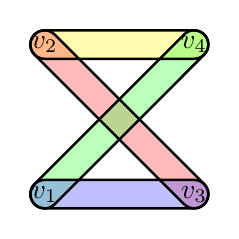
\begin{tikzpicture}[x=0.95cm,y=0.95cm]
  \fill[yellow!80, fill opacity=0.38] (0.000,2.190) arc[start angle=90.00, end angle=270.00, radius=0.19] -- (2.000,1.810) arc[start angle=-90.00, end angle=90.00, radius=0.19] -- cycle;
  \fill[red!70, fill opacity=0.38] (0.134,2.134) arc[start angle=45.00, end angle=225.00, radius=0.19] -- (1.866,-0.134) arc[start angle=-135.00, end angle=45.00, radius=0.19] -- cycle;
  \fill[green!70, fill opacity=0.38] (-0.134,0.134) arc[start angle=135.00, end angle=315.00, radius=0.19] -- (2.134,1.866) arc[start angle=-45.00, end angle=135.00, radius=0.19] -- cycle;
  \fill[blue!65, fill opacity=0.38] (0.000,0.190) arc[start angle=90.00, end angle=270.00, radius=0.19] -- (2.000,-0.190) arc[start angle=-90.00, end angle=90.00, radius=0.19] -- cycle;
  \draw[black, line width=0.9pt] (0.000,2.190) arc[start angle=90.00, end angle=270.00, radius=0.19] -- (2.000,1.810) arc[start angle=-90.00, end angle=90.00, radius=0.19] -- cycle;
  \draw[black, line width=0.9pt] (0.134,2.134) arc[start angle=45.00, end angle=225.00, radius=0.19] -- (1.866,-0.134) arc[start angle=-135.00, end angle=45.00, radius=0.19] -- cycle;
  \draw[black, line width=0.9pt] (-0.134,0.134) arc[start angle=135.00, end angle=315.00, radius=0.19] -- (2.134,1.866) arc[start angle=-45.00, end angle=135.00, radius=0.19] -- cycle;
  \draw[black, line width=0.9pt] (0.000,0.190) arc[start angle=90.00, end angle=270.00, radius=0.19] -- (2.000,-0.190) arc[start angle=-90.00, end angle=90.00, radius=0.19] -- cycle;
  \node[inner sep=0pt] at (0.000,2.000) {$v_{2}$};
  \node[inner sep=0pt] at (2.000,2.000) {$v_{4}$};
  \node[inner sep=0pt] at (0.000,0.000) {$v_{1}$};
  \node[inner sep=0pt] at (2.000,0.000) {$v_{3}$};
\end{tikzpicture}
\caption{Hypergraph $C_4$}\end{subfigure}\hfill
\begin{subfigure}{0.45\linewidth}\centering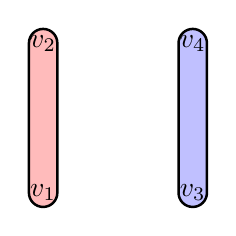
\begin{tikzpicture}[x=0.95cm,y=0.95cm]
  \fill[red!70, fill opacity=0.38] (-0.190,0.000) arc[start angle=180.00, end angle=360.00, radius=0.19] -- (0.190,2.000) arc[start angle=0.00, end angle=180.00, radius=0.19] -- cycle;
  \fill[blue!65, fill opacity=0.38] (1.810,0.000) arc[start angle=180.00, end angle=360.00, radius=0.19] -- (2.190,2.000) arc[start angle=0.00, end angle=180.00, radius=0.19] -- cycle;
  \draw[black, line width=0.9pt] (-0.190,0.000) arc[start angle=180.00, end angle=360.00, radius=0.19] -- (0.190,2.000) arc[start angle=0.00, end angle=180.00, radius=0.19] -- cycle;
  \draw[black, line width=0.9pt] (1.810,0.000) arc[start angle=180.00, end angle=360.00, radius=0.19] -- (2.190,2.000) arc[start angle=0.00, end angle=180.00, radius=0.19] -- cycle;
  \node[inner sep=0pt] at (0.000,2.000) {$v_{2}$};
  \node[inner sep=0pt] at (2.000,2.000) {$v_{4}$};
  \node[inner sep=0pt] at (0.000,0.000) {$v_{1}$};
  \node[inner sep=0pt] at (2.000,0.000) {$v_{3}$};
\end{tikzpicture}
\caption{Transversal of $C_4$}\end{subfigure}
\caption{Hypergraph $K_2^{\cdot\cdot}$ and its transversal. Hypergraph $C_4$ and its transversal.}\label{fig:k2dd-c4}
\end{figure}

\begin{figure}[tp]
\centering
\begin{subfigure}{0.45\linewidth}\centering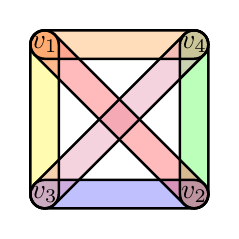
\begin{tikzpicture}[x=0.95cm,y=0.95cm]
  \fill[orange!70, fill opacity=0.38] (0.000,2.190) arc[start angle=90.00, end angle=270.00, radius=0.19] -- (2.000,1.810) arc[start angle=-90.00, end angle=90.00, radius=0.19] -- cycle;
  \fill[yellow!80, fill opacity=0.38] (-0.190,0.000) arc[start angle=180.00, end angle=360.00, radius=0.19] -- (0.190,2.000) arc[start angle=0.00, end angle=180.00, radius=0.19] -- cycle;
  \fill[green!70, fill opacity=0.38] (1.810,0.000) arc[start angle=180.00, end angle=360.00, radius=0.19] -- (2.190,2.000) arc[start angle=0.00, end angle=180.00, radius=0.19] -- cycle;
  \fill[blue!65, fill opacity=0.38] (0.000,0.190) arc[start angle=90.00, end angle=270.00, radius=0.19] -- (2.000,-0.190) arc[start angle=-90.00, end angle=90.00, radius=0.19] -- cycle;
  \fill[red!70, fill opacity=0.38] (0.134,2.134) arc[start angle=45.00, end angle=225.00, radius=0.19] -- (1.866,-0.134) arc[start angle=-135.00, end angle=45.00, radius=0.19] -- cycle;
  \fill[purple!45, fill opacity=0.38] (-0.134,0.134) arc[start angle=135.00, end angle=315.00, radius=0.19] -- (2.134,1.866) arc[start angle=-45.00, end angle=135.00, radius=0.19] -- cycle;
  \draw[black, line width=0.9pt] (0.000,2.190) arc[start angle=90.00, end angle=270.00, radius=0.19] -- (2.000,1.810) arc[start angle=-90.00, end angle=90.00, radius=0.19] -- cycle;
  \draw[black, line width=0.9pt] (-0.190,0.000) arc[start angle=180.00, end angle=360.00, radius=0.19] -- (0.190,2.000) arc[start angle=0.00, end angle=180.00, radius=0.19] -- cycle;
  \draw[black, line width=0.9pt] (1.810,0.000) arc[start angle=180.00, end angle=360.00, radius=0.19] -- (2.190,2.000) arc[start angle=0.00, end angle=180.00, radius=0.19] -- cycle;
  \draw[black, line width=0.9pt] (0.000,0.190) arc[start angle=90.00, end angle=270.00, radius=0.19] -- (2.000,-0.190) arc[start angle=-90.00, end angle=90.00, radius=0.19] -- cycle;
  \draw[black, line width=0.9pt] (0.134,2.134) arc[start angle=45.00, end angle=225.00, radius=0.19] -- (1.866,-0.134) arc[start angle=-135.00, end angle=45.00, radius=0.19] -- cycle;
  \draw[black, line width=0.9pt] (-0.134,0.134) arc[start angle=135.00, end angle=315.00, radius=0.19] -- (2.134,1.866) arc[start angle=-45.00, end angle=135.00, radius=0.19] -- cycle;
  \node[inner sep=0pt] at (0.000,2.000) {$v_{1}$};
  \node[inner sep=0pt] at (2.000,2.000) {$v_{4}$};
  \node[inner sep=0pt] at (0.000,0.000) {$v_{3}$};
  \node[inner sep=0pt] at (2.000,0.000) {$v_{2}$};
\end{tikzpicture}
\caption{Hypergraph $K_4$}\end{subfigure}\hfill
\begin{subfigure}{0.45\linewidth}\centering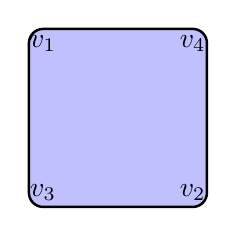
\begin{tikzpicture}[x=0.95cm,y=0.95cm]
  \fill[blue!65, fill opacity=0.38] (-0.190,0.000) arc[start angle=180.00, end angle=270.00, radius=0.19] -- (2.000,-0.190) arc[start angle=-90.00, end angle=0.00, radius=0.19] -- (2.190,2.000) arc[start angle=0.00, end angle=90.00, radius=0.19] -- (0.000,2.190) arc[start angle=90.00, end angle=180.00, radius=0.19] -- cycle;
  \draw[black, line width=0.9pt] (-0.190,0.000) arc[start angle=180.00, end angle=270.00, radius=0.19] -- (2.000,-0.190) arc[start angle=-90.00, end angle=0.00, radius=0.19] -- (2.190,2.000) arc[start angle=0.00, end angle=90.00, radius=0.19] -- (0.000,2.190) arc[start angle=90.00, end angle=180.00, radius=0.19] -- cycle;
  \node[inner sep=0pt] at (0.000,2.000) {$v_{1}$};
  \node[inner sep=0pt] at (2.000,2.000) {$v_{4}$};
  \node[inner sep=0pt] at (0.000,0.000) {$v_{3}$};
  \node[inner sep=0pt] at (2.000,0.000) {$v_{2}$};
\end{tikzpicture}
\caption{Transversal of $K_4$}\end{subfigure}
\caption{Hypergraph $K_4$ and its transversal.}\label{fig:k4}
\end{figure}

\section{Impact of \FKA{} on Symmetry}

We can understand how the symmetry within the hypergraph gets impacted when \FKA{} decomposes and recurses on input hypergraphs $G$, $H$ to test whether they are mutually transversals or not from the following discussion.

\begin{lemma}\label{lem:aut-tr}
Suppose $\Aut(H)=\mathcal{G}$ for a hypergraph $H$ and its transversal hypergraph is denoted $\Tr(H)$. Then $\Aut(\Tr(H))\cong\mathcal{G}$.
\end{lemma}

\begin{proof}
Suppose not. Let $\mathcal{G}'=\Aut(\Tr(H))$, and assume $\mathcal{G}\neq\mathcal{G}'$. Then there exists an automorphism $\phi$ such that either $\phi\in\mathcal{G}$ but $\phi\notin\mathcal{G}'$, or $\phi\in\mathcal{G}'$ but $\phi\notin\mathcal{G}$.

Suppose $\phi\in\mathcal{G}$ but $\phi\notin\mathcal{G}'$. Since $\phi\in\mathcal{G}$, it preserves the edge structure of $H$, mapping each hyperedge $e\in E(H)$ to another hyperedge $\phi(e)\in E(H)$. Now, for any minimal transversal $t\in\Tr(H)$, $\phi(t)$ intersects every hyperedge $\phi(e)$ of $H$, and as $\phi$ is a bijection, $\phi(t)$ remains minimal. Thus, $\phi(t)\in\Tr(H)$, implying $\phi\in\mathcal{G}'$, which contradicts the assumption.

A similar argument applies if $\phi\in\mathcal{G}'$ but $\phi\notin\mathcal{G}$. Hence, $\mathcal{G}=\mathcal{G}'$.
\end{proof}

\begin{lemma}\label{lem:break}
In \FKA, the recursive decomposition on the most frequent vertex $v_i$ eliminates all symmetries associated with $v_i$ in the hypergraphs $H$ and $\Tr(H)$ by ensuring that any automorphism generators including $v_i$ are removed. As a result, all nontrivial automorphism generators that include $v_i$ are removed.
\end{lemma}

\begin{proof}
Let $H=(V,E)$ and $\Tr(H)=(V,E')$ be Sperner hypergraphs with a common vertex set $V$, where $E=\{e_1,e_2,\dots\}$ and $E'=\{t_1,t_2,\dots\}$ represent the edge sets of $H$ and $\Tr(H)$, respectively. Suppose $|H|\cdot|\Tr(H)|\geq 2$, and let $v_i$ be the most frequent vertex, occurring in either $H$ or $\Tr(H)$ with frequency at least $\frac{1}{\log(|H|+|\Tr(H)|)}$. Assume there exists a nontrivial automorphism generator $\sigma$ acting on both $H$ and $\Tr(H)$.

By definition, $\sigma$ is an automorphism generator, creating other automorphisms through composition, and it induces a permutation of vertices that forms nontrivial orbits within $V$. These orbits represent structural dependencies among vertices, as vertices within the same orbit are indistinguishable under the automorphisms generated by $\sigma$. The \FKA{} decomposition selects $v_i$, the most frequent vertex, and deletes it, effectively breaking the generator $\sigma$.

If $v_i$ is part of multiple automorphism generators, its removal disrupts the composition of these generators. Specifically, for a generator such as $(ab)(cd)$, deleting $v_i=a$ removes $a$ from the orbit, effectively separating the generator into $(cd)$. This action breaks the combined structure of the generators, rendering automorphisms generated through their composition invalid. As a result, all symmetries dependent on $v_i$ collapse, ensuring that no nontrivial automorphisms involving $v_i$ remain in the decomposed hypergraphs.
\end{proof}

\begin{lemma}\label{lem:independent}
Let $H$ and $\Tr(H)$ be transversal hypergraphs with vertex set $V$. Suppose $v_i$ and $v_j$ are distinct vertices of $H$, and let $\sigma$ be an automorphism generator of $H$. If $v_i$ and $v_j$ do not belong to the same transposition of vertices within $\sigma$, deleting $v_i$ does not affect symmetries involving $v_j$. Specifically, if $\sigma\cong\langle(v_i\,v_k)(v_j\,v_m)\rangle$, removing $v_i$ breaks transpositions involving $v_i$, such as $(v_iv_k)$ from all automorphisms in $\Aut(H)$, but leaves other transpositions like $(v_jv_m)$ intact, preserving symmetries associated with $v_j$.
\end{lemma}

\begin{proof}
Let $H=(V,E)$ and $\Tr(H)=(V,E')$ be Sperner hypergraphs that are transversal to each other. Consider distinct vertices $v_i$ and $v_j$ in $V$, and let $\sigma$ be an automorphism generator of $H$. The relationship between $v_i$ and $v_j$ within $\sigma$ can be described as the following:

If $v_i$ and $v_j$ are in the same transposition within $\sigma$, such as $\sigma\cong\langle(v_i\,v_j)\rangle$, removing $v_i$ directly breaks the transposition $(v_i\,v_j)$. This action invalidates all automorphisms involving both $v_i$ and $v_j$, as their symmetry depends entirely on the transposition $(v_i\,v_j)$. The decomposition, therefore, eliminates all symmetries related to $v_j$ in this case.

If $v_i$ and $v_j$ are in different transpositions within the same generator, such as $\sigma\cong\langle(v_i\,v_k)(v_j\,v_m)\rangle$, the transpositions $(v_i\,v_k)$ and $(v_j\,v_m)$ are independent. Removing $v_i$ invalidates all automorphisms generated by $(v_i\,v_k)$ but does not affect the ones generated by $(v_j\,v_m)$. In this case, the decomposition breaks automorphisms involving $v_i$ while leaving all symmetries associated with $v_j$ intact.

If $v_i$ and $v_j$ belong to different generators, such as $\sigma_1\cong\langle(v_i\,v_k)\rangle$ and $\sigma_2\cong\langle(v_j\,v_m)\rangle$, the automorphic structures of $v_i$ and $v_j$ are completely independent. Removing $v_i$ affects only $\sigma_1$ by breaking $(v_i\,v_k)$, while $\sigma_2$ and its transposition $(v_j\,v_m)$ remain unaffected. The decomposition, in this case, does not impact the symmetries involving $v_j$.

Thus, in \FKA{} decomposition, removing $v_i$ breaks symmetries involving $v_i$ while preserving those associated with $v_j$, provided $v_i$ and $v_j$ are not part of the same transposition.
\end{proof}

\begin{corollary}\label{cor:aut-min}
Let $min(H)$ be the Sperner reduced hypergraph of $H$ (\ref{def:sperner-reduction}). Then $\Aut(H)\cong\Aut(min(H))$.
\end{corollary}

\begin{proof}
Consider the Sperner reduced hypergraph $min(H)=(V,E)$. Let's show that if $\sigma\in\Aut(H)$, then $\sigma\in\Aut(min(H))$. By definition, $\sigma\in\Aut(H)$ maps each hyperedge in $E(H)$ to another hyperedge in $E(H)$. For any $e_i\in E_{min}(H)$, $\sigma(e_i)$ must also belong to $E(H)$. Suppose $\sigma(e_i)\notin E_{min}(H)$; then there exists $e_j\in E(H)$ such that $e_j\subset\sigma(e_i)$. Applying $\sigma^{-1}$, this implies $\sigma^{-1}(e_j)\subset e_i$, contradicting the minimality of $e_i$ in $min(H)$. Thus, $\sigma(e_i)\in E_{min}(H)$, proving that $\sigma$ preserves minimal hyperedges, so $\sigma\in\Aut(min(H))$.

Now, suppose that $\sigma\in\Aut(min(H))$. Then, it ensures that $\sigma$ maps each minimal hyperedge $e_i\in E_{min}(H)$ to another minimal hyperedge in $E_{min}(H)$. For any $e_i\in E(H)$, if $e_i\in E_{min}(H)$, then $\sigma(e_i)\in E_{min}(H)\subset E(H)$. If $e_i\notin E_{min}(H)$, $e_i$ must be a superset of some $e_j\in E_{min}(H)$. Since $\sigma$ preserves $E_{min}(H)$, $\sigma(e_j)\in E_{min}(H)$, making $\sigma(e_i)$ a superset of $\sigma(e_j)$ and ensuring $\sigma(e_i)\in E(H)$. Therefore, $\sigma(E(H))=E(H)$, and $\sigma\in\Aut(H)$.

Thus, $\Aut(H)\cong\Aut(min(H))$.
\end{proof}

\section{Primal Graph of A Hypergraph and \FKA{} Recursion}

\begin{definition}
The \emph{primal graph} of a hypergraph $H=(V,E)$, denoted $G(H)$, is the graph with the same vertex set $V$, where two vertices $u,v\in V$ are adjacent if and only if they appear together in at least one hyperedge $e\in E$.
\end{definition}

Primal graphs are also known as co-occurrence graphs, [2]-sections of hypergraphs, and Gaifman graphs in the literature \cite{DPP18}.

\begin{definition}
A hypergraph $H=(V,E(H))$ is \emph{conformal} if every maximal clique in its primal graph $G(H)$ is a hyperedge of $H$.
\end{definition}

For a conformal hypergraph $H=(V,E)$ and its primal graph $G(H)$, the clique hypergraph of $G(H)$ (\ref{def:clique-missing}) is exactly $H$. Primal graph of a hypergraph represents the symmetric and structural properties of the hypergraph rather faithfully for conformal hypergraphs, as $G$ is uniquely determined if and only if $H$ is conformal. \cite{GMR06}. Since for conformal hypergraphs, every maximal clique in $G$ corresponds to a hyperedge in $H$, analyzing the cliques of $G$ can reveal key properties about hypergraph. For general hypergraphs, the primal graph $G$ does not uniquely determine it because multiple hypergraphs can share the same primal graph. The hyperedges of a general hypergraph may involve overlapping edges where the primal graph cannot distinguish the separate edges from the cliques of $G$.

With conformality, looking at the primal graph and how they they interact through the \FKA{} recursion can give us an insight into whether the induced subgraph preserved or display any characteristics through the decomposition. Graph minor operations are a well-known method to generate induced subgraphs from a graph. Generalizing this for hypergraphs, we get:

A hypergraph $H'$ is a \emph{minor} of $H$, denoted $H'\preceq H$, if $H'$ is obtained by:
\begin{itemize}
\item Deleting a vertex.
\item Deleting proper subhyperedges $e_j\subset e_i$, $e_i\in E(H)$.
\item Shrinking a 2-edge (adjacent vertices in $G(H)$) into a single vertex.
\end{itemize}

For a pair of Sperner hypergraphs $(F,H)$, the \emph{contraction} (\ref{def:contraction}) of $v\in V(F)$ results in:
\begin{align*}
F'&=\left(V(F)\setminus\{v\},\{e_i=e_j\setminus\{v\}\mid e_j\in E(F)\}\right),\\
H'&=\left(V(F)\cap V(H)\setminus\{v\},\{e_i=e_j\setminus\{v\}\mid e_j\in E(H)\cap V(F)\}\right).
\end{align*}
If $V(F)=V(H)=V$, this simplifies to:
\begin{align*}
F'&=\left(V\setminus\{v\},\{e_i=e_j\setminus\{v\}\mid e_j\in E(F)\}\right),\\
H'&=\left(V\setminus\{v\},\{e_i=e_j\setminus\{v\}\mid e_j\in E(H)\}\right).
\end{align*}

The \emph{deletion} (\ref{def:deletion}) of $v$ results in:
\begin{align*}
F'&=\left(V\setminus\{v\},\{e_i\in E(F)\mid v\notin e_i\}\right),\\
H'&=\left(V\setminus\{v\},\{e_i=e_j\setminus\{v\}\mid e_j\in E(H)\}\right).
\end{align*}
\cite{BS15}.

A \textbf{minor map} $\mu:F\to F'$ satisfies the following:
\begin{itemize}
\item $\mu(v)\cap\mu(u)=\emptyset$ for all distinct $u,v\in V(F)$,
\item $\{v\in V(F)\mid\mu(v)\cap e_j\neq\emptyset\}\subseteq e_i$ or $\emptyset$, for some $e_i\in E(F)$, for all $e_j\in E(F')$.
\end{itemize}

$F'\preceq F$ if and only if there exists $\mu$ such that $F'$ is formed as:
\[
F'=\bigcup_{v\in V(F')}F[\mu(v)]\cup\bigcup_{e\in E(F)}\mu(e).
\]

For hypergraph pairs $(F,H)$ and $(F',H')$, $(F,H)\preceq(F',H')$ if and only if there exists a minor map $\mu:(F,H)\to(F',H')$.

Therefore, minor operations on a hypergraph $H$ extends to its primal graph, denoted $G(H)$. However, the converse does not hold, as primal graphs do not fully preserve hypergraph structure.

\begin{example}
Let $H=(V,E)$ be a Sperner hypergraph where $V=\{v_1,v_2,v_3,v_4\}$ and $E=\{e_1,e_2,e_3\}$ with:
\[
e_1=\{v_1,v_2,v_3\},\quad e_2=\{v_2,v_4\},\quad e_3=\{v_3,v_4\}.
\]
The primal graph $G(H)$ has vertex set $V$ and edges:
\[
\{v_1,v_2\},\{v_1,v_3\},\{v_2,v_3\},\{v_2,v_4\},\{v_3,v_4\}.
\]

Consider the automorphism $\alpha\in\Aut(G(H))$ defined as:
\[
\alpha(v_1)=v_3,\quad\alpha(v_2)=v_2,\quad\alpha(v_3)=v_1,\quad\alpha(v_4)=v_4.
\]

This permutation preserves adjacency in $G(H)$ but maps the hyperedges of $H$ as:
\[
\alpha(e_1)=\{v_3,v_2,v_1\},\quad\alpha(e_2)=\{v_2,v_4\},\quad\alpha(e_3)=\{v_1,v_4\}.
\]
While $\alpha$ is valid in $G(H)$, it fails to preserve the hyperedge structure of $H$. Thus, $\alpha\in\Aut(G(H))$, but $\alpha\notin\Aut(H)$.
\end{example}

\cite{AGT12} established the connection between hypergraph minors and their primal graphs with the following lemma:

\begin{lemma}
For Sperner hypergraphs $H,H'$, $H'\preceq H\iff(G(H'),H')\preceq(G(H),H)$.
\end{lemma}

To illustrate this, let the hypergraphs $G^{\emptyset}$ and $G^1$ be defined as:
\[
G^{\emptyset}=(V,\emptyset),\quad G^1=(V,E(G^1)),\quad E(G^1)=\{\{v\}\mid v\in V\}.
\]
Here, $G^{\emptyset}$ corresponds to the empty hypergraph, and $G^1$ corresponds to the singleton hypergraph, where each edge contains a single vertex. For any two graphs $G(H)$ and $G(H')$, the following equivalence holds:
\[
G(H')\preceq G(H)\iff(G(H'),G(H')^{\emptyset})\preceq(G(H),G(H)^{\emptyset})\iff(G(H'),G(H')^1)\preceq(G(H),G(H)^1).
\]
This demonstrates that hypergraph minor operations extend to their primal graphs. Therefore, we note the following:

\begin{observation}
The \FKA{} recursive decomposition method induces a minor map between the primal graph of input hypergraphs and their induced subhypergraphs.
\end{observation}

The \FKA{} algorithm recursively decomposes input hypergraphs $F$ and $H$ into subproblems corresponding to the contraction and deletion subhypergraphs $F'$ and $H'$. These operations extend to the primal graphs $G(F)$ and $G(H)$, resulting in the minors $G(F')$ and $G(H')$.

The decomposition proceeds until reaching end states: the empty graph $G^{\emptyset}=(V,\emptyset)$ and the singleton hypergraph $G^1=(V,E(G^1))$, where $E(G^1)=\{\{v\}\mid v\in V\}$.

In the next chapters, we explore the primal graph structures of poorly performing hypergraph classes in \FKA, examining their symmetry and properties preserved during decomposition.

\section{Symmetry in \FKA{} Recursion}

\FKA{} recursion process involves a decomposition, creating two smaller subproblems. To understand the effect of this operation on the symmetric structure of the input hypergraphs, it suffices to analyze the symmetry of one of the input hypergraphs, say $G$. By transversality, the other hypergraph $H$ will inherit symmetry restrictions from $G$. Depending on whether the input hypergraphs $G$ and $H$ have a nontrivial automorphism group and the choice of the vertex $v_i$, hypergraphs in \FKA{} recursion can gain symmetry, lose symmetry, or no changes in symmetry.

The minor operation \textbf{L} applied to $G$ produces a subhypergraph $G_1$ by deleting a vertex $v_i$ and all hyperedges incident to it while \textbf{R} contains $G_0\vee G_1$. Looking at the symmetric changes in \textbf{L} on $G$ to get $G_1$ is sufficient considering a similar operation can be described for $H$ and $H_1$ which is the transversal of $G_0\vee G_1$ and has the same symmetry. This operation can affect the automorphism group of $G$ in three distinct ways:

First, the hypergraph can \emph{gain} symmetry. Suppose $G_1$ has a new automorphism $\sigma$ such that $\sigma\notin\Aut(G)$. For $\sigma$ to permute two vertices $u,v\in V(G_1)$, the deletion of $v_i$ must remove hyperedges that previously prevented this symmetry. Specifically, in the hyperedges of $G$ incident to $v_i$, there must exist a structural conflict where $\sigma(u)\neq v$, meaning $u$ and $v$ were distinguished in $G$ but become indistinguishable in $G_1$ after the removal of $v_i$. This situation leads to a larger automorphism group for $G_1$ compared to $G$.

Second, the hypergraph can \emph{lose} symmetry. Suppose $G$ has a nontrivial automorphism group, and $\sigma\in\Aut(G)$. If $v_i$ participates in transpositions or permutations that are part of a generator of $\Aut(G)$, then removing $v_i$ invalidates all symmetries involving $v_i$. For example, if $\sigma$ contains a transposition $(v_i\,u)$, deleting $v_i$ disrupts the symmetry, reducing the automorphism group of $G_1$ to a subgroup of $\Aut(G)$. This case is rigorously outlined in \ref{lem:break}.

Finally, the symmetry of the hypergraph may remain \emph{unchanged}. If the vertex $v_i$ being removed does not participate in any transpositions within the automorphism group of $G$, the automorphism group of $G_1$ will be identical to $\Aut(G)$. This is explained in \ref{lem:independent}.

Understanding the nature of induced symmetries during \FKA{} recursion is challenging due to their hierarchical and modular structure. As we can see, depending on the choice of vertex, a variety of symmetries or no symmetries might emerge.
